\chapter{Algoritmi}
\label{ch:algoritmi}

U ovom poglavlju teorijski su obrađena tri algoritma koja čine jezgro realizovanog akceleratora, redosledom kojim učestvuju u hibridnom protokolu iz odeljka \ref{sec:hibridni_sistem}: ECDH protokol za razmenu ključeva, SHA-3 heš funkcija i AES algoritam u GCM režimu rada. Za svaki algoritam dat je matematički okvir, opis same konstrukcije i svojstva bitna za hardversku realizaciju, koja je predmet poglavlja \ref{ch:hardver}. Matematičke osnove konačnih polja, zajedničke za sva tri algoritma, sistematizovane su u dodatku \ref{app:math}.

\section{ECDH -- razmena ključeva na eliptičkim krivama}
\label{sec:ecdh}

\subsection{Diffie--Hellmanov protokol}
\label{subsec:dh_protokol}

Diffie--Hellmanov protokol \cite{diffie_hellman} omogućava dvema stranama da preko javnog kanala uspostave zajedničku tajnu. Ideja protokola je nezavisna od konkretne matematičke strukture. Potrebna je grupa u kojoj je eksponencijacija (uzastopna primena grupovne operacije) laka, a njena inverzija, problem diskretnog logaritma, praktično nerešiva. U izvornom obliku protokol koristi multiplikativnu grupu ostataka po modulu velikog prostog broja. Vremenom su, međutim, za ovu grupu razvijeni subeksponencijalni algoritmi za diskretni logaritam, što zahteva sve veće dužine ključeva. Eliptičke krive nude grupu za koju takvi algoritmi nisu poznati, pa se ekvivalentna sigurnost postiže znatno kraćim ključevima.

\subsection{Eliptičke krive}
\label{subsec:elipticke_krive}

Eliptička kriva nad poljem $K$ je skup rešenja jednačine trećeg stepena u dve promenljive, proširen posebnom tačkom u beskonačnosti $\mathcal{O}$. Nad poljima karakteristike različite od 2 i 3 jednačina se svodi na kratki Vajerštrasov (engl. \textit{Weierstrass}) oblik:
\begin{equation}
    y^2 = x^3 + ax + b.
\end{equation}
Nad binarnim poljima $\mathrm{GF}(2^m)$, koja su korišćena u ovom radu, nesupersingularna eliptička kriva ima oblik:
\begin{equation}
    E:\; y^2 + xy = x^3 + ax^2 + b, \qquad a, b \in \mathrm{GF}(2^m),\; b \neq 0.
    \label{eq:binarna_kriva}
\end{equation}
\smallbreak
Ključno svojstvo eliptičkih krivih je da se nad skupom njihovih tačaka može definisati operacija sabiranja koja taj skup čini Abelovom grupom, sa tačkom $\mathcal{O}$ kao neutralnim elementom. Geometrijski, zbir tačaka $P$ i $Q$ dobija se tako što se kroz njih povuče prava. Ona seče krivu u još tačno jednoj tački, čijom se refleksijom u odnosu na $x$-osu dobija $P+Q$, kako je prikazano na slici \ref{fig:ec_sabiranje}. Prikaz je dat nad realnim brojevima, gde je geometrija očigledna. Nad konačnim poljem geometrijska intuicija se gubi, ali važe iste algebarske formule.

\begin{figure}[H]
\centering
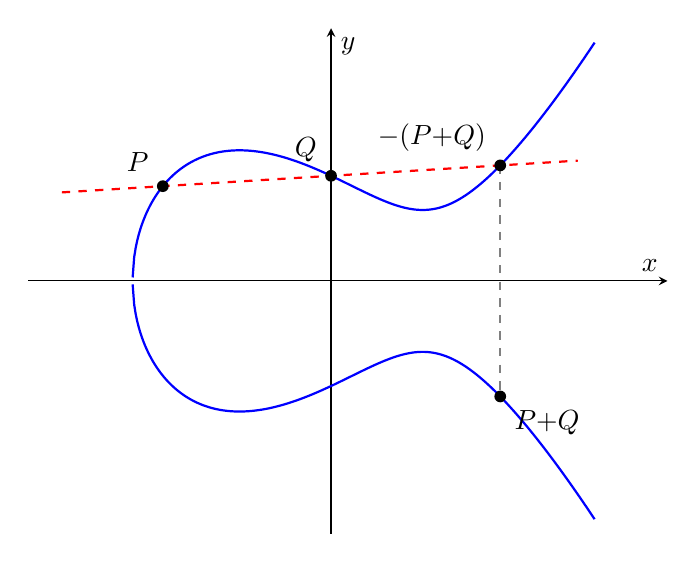
\begin{tikzpicture}
\begin{axis}[width=0.8\textwidth, height=8cm, axis lines=middle, xlabel=$x$, ylabel=$y$,
             xmin=-2.7, xmax=3.0, ymin=-3.4, ymax=3.4, ticks=none, clip=false]
  \addplot[domain=-1.769:2.35, samples=300, thick, blue] {sqrt(x^3-2*x+2)};
  \addplot[domain=-1.769:2.35, samples=300, thick, blue] {-sqrt(x^3-2*x+2)};
  \addplot[domain=-2.4:2.2, dashed, thick, red] {1.41421+0.09294*x};
  \draw[dashed, thick, gray] (axis cs:1.5086,1.5544) -- (axis cs:1.5086,-1.5544);
  \node[circle, fill=black, inner sep=1.5pt, label={above left:$P$}] at (axis cs:-1.5,1.2748) {};
  \node[circle, fill=black, inner sep=1.5pt, label={above left:$Q$}] at (axis cs:0,1.41421) {};
  \node[circle, fill=black, inner sep=1.5pt, label={above left:$-(P{+}Q)$}] at (axis cs:1.5086,1.5544) {};
  \node[circle, fill=black, inner sep=1.5pt, label={below right:$P{+}Q$}] at (axis cs:1.5086,-1.5544) {};
\end{axis}
\end{tikzpicture}
\caption{Geometrijsko sabiranje tačaka na eliptičkoj krivoj (prikaz nad realnim brojevima)}
\label{fig:ec_sabiranje}
\end{figure}

Algebarski, za krivu oblika (\ref{eq:binarna_kriva}) i tačke $P=(x_1, y_1)$ i $Q=(x_2, y_2)$, $P \neq \pm Q$, zbir $P+Q=(x_3, y_3)$ računa se kao:
\begin{equation}
    \lambda = \frac{y_1 + y_2}{x_1 + x_2}, \qquad
    x_3 = \lambda^2 + \lambda + x_1 + x_2 + a, \qquad
    y_3 = \lambda(x_1 + x_3) + x_3 + y_1,
    \label{eq:point_add}
\end{equation}
dok se dupliranje tačke $2P=(x_3,y_3)$ računa kao:
\begin{equation}
    \lambda = x_1 + \frac{y_1}{x_1}, \qquad
    x_3 = \lambda^2 + \lambda + a, \qquad
    y_3 = x_1^2 + (\lambda + 1)\,x_3.
    \label{eq:point_double}
\end{equation}
Sve operacije u izrazima (\ref{eq:point_add}) i (\ref{eq:point_double}) su operacije u polju $\mathrm{GF}(2^m)$. Sabiranje i oduzimanje se u polju karakteristike 2 poklapaju. Formule pokazuju da se aritmetika tačaka svodi na četiri osnovne operacije u polju: sabiranje, množenje, kvadriranje i inverziju, što neposredno određuje strukturu hardverske aritmetičke jedinice \cite{hankerson}.

\subsection{Binarno polje \texorpdfstring{$\mathrm{GF}(2^m)$}{GF(2\^{}m)}}
\label{subsec:binarno_polje}

Elementi polja $\mathrm{GF}(2^m)$ mogu se predstaviti kao polinomi stepena manjeg od $m$ sa koeficijentima u $\mathrm{GF}(2)=\{0,1\}$, odnosno kao binarne reči dužine $m$ bitova u polinomijalnoj bazi. Aritmetika se obavlja po modulu nesvodljivog polinoma $f(x)$ stepena $m$:
\begin{itemize}[itemsep=2pt]
    \item Sabiranje je sabiranje koeficijenata po modulu 2, dakle bitska operacija isključivo-ili (XOR) u jednom logičkom nivou.
    \item Množenje je množenje polinoma praćeno redukcijom po modulu $f(x)$. Ovo je dominantna operacija i po broju izvršavanja i po hardverskoj ceni, pa izbor arhitekture množača presudno određuje odnos površine i brzine celog sistema. Taj izbor je pitanje realizacije.
    \item Kvadriranje je znatno jeftinije od opšteg množenja, jer se kvadriranjem polinoma koeficijenti samo ``razmaknu'' ($x^i \mapsto x^{2i}$), pa se operacija svodi na umetanje nula i fiksnu redukciju, čistu kombinacionu mrežu.
    \item Inverzija je najskuplja operacija. Računa se proširenim Euklidovim algoritmom ili lancem kvadriranja i množenja, jer se svodi na stepenovanje unapred poznatim eksponentom (odeljak \ref{subsec:gf571_aritmetika}). U praksi se algoritmi biraju tako da broj inverzija bude sveden na minimum, o čemu je reč u odeljku \ref{subsec:montgomery}.
\end{itemize}
\smallbreak
Prednost binarnih polja za hardversku realizaciju je u tome što je aritmetika bez prenosa (engl. \textit{carry-free}), pa nema lanaca prenosa koji ograničavaju radnu učestanost, a sve operacije se prirodno preslikavaju na XOR i AND mreže.

\subsection{Kriva B-571}
\label{subsec:b571}

U radu je korišćena kriva B-571, čiji su parametri dati NIST preporukom SP 800-186 \cite{sp800186}. Kriva je oblika (\ref{eq:binarna_kriva}) nad poljem $\mathrm{GF}(2^{571})$ sa redukcionim polinomom:
\begin{equation}
    f(x) = x^{571} + x^{10} + x^5 + x^2 + 1,
\end{equation}
koeficijentom $a=1$ i pseudoslučajno generisanim koeficijentom $b$ čija je vrednost data u standardu. Red osnovne tačke $G$ je prost broj $n$ dužine 570 bitova, a kofaktor krive je $h=2$. B-571 je najveća standardizovana binarna kriva i pruža sigurnosni nivo od približno 285 bitova. Kompletne vrednosti parametara krive ($b$, koordinate tačke $G$, red $n$) date su u dodatku \ref{app:b571}.
\smallbreak
Uz izbor ove krive ide i jedna napomena. Ista preporuka \cite{sp800186} sve krive nad binarnim poljima, pa i B-571, označava kao prevaziđene (engl. \textit{deprecated}) za nove primene i za njih preporučuje krive nad prostim poljima. Preporuka pritom ne navodi nijednu poznatu bezbednosnu slabost ovih krivih. Razlog povlačenja je isključivo slaba rasprostranjenost u praksi, a najbolji poznati napadi na ECDLP nad njima ostaju generički, kao i kod krivih nad prostim poljima. Kriva je u ovom radu ipak izabrana iz hardverskih razloga, obrazloženih u uvodu odeljka \ref{sec:hw_ecdh}.

\subsection{Inverzija: Itoh--Tsujiijeva metoda}
\label{subsec:gf571_aritmetika}

Od četiri operacije iz odeljka \ref{subsec:binarno_polje} inverzija je jedina koja se ne računa neposredno, ali se algoritamski svodi na preostale. Multiplikativna grupa polja $\mathrm{GF}(2^m)$ ima $2^m - 1$ elemenata, pa za svako $u \neq 0$ važi $u^{2^m - 1} = 1$, odnosno $u^{-1} = u^{2^m - 2}$, dakle inverzija je stepenovanje unapred poznatim eksponentom.
\smallbreak
Eksponent $2^m - 2$ u binarnom zapisu čini niz od $m-1$ jedinice praćen nulom. Opšti postupak kvadriraj-i-množi troši po jedno množenje na svaku jedinicu eksponenta sem vodeće, pa bi ovde tražio $m-2$ množenja, za B-571 čak 569. Upravo pravilnost eksponenta nudi izlaz. Niz jedinica ne mora da se gradi jedinicu po jedinicu, jer se dva već izgrađena niza spajaju jednim množenjem. Taj put sledi Itoh--Tsujiijeva metoda \cite{itoh_tsujii}, koja traženi eksponent gradi kao adicioni lanac. Metoda je prvobitno data za normalne baze. Na polinomijalnu bazu, koja se koristi u ovom radu, preneli su je Guajardo i Paar \cite{guajardo_paar}. Uvodi se pomoćna veličina
\begin{equation}
    \beta_t = u^{\,2^t - 1},
    \label{eq:itoh_beta}
\end{equation}
čiji eksponent u binarnom zapisu čini $t$ uzastopnih jedinica, i za nju važe dve veze:
\begin{equation}
    \beta_{2t} = \left(\beta_t\right)^{2^t} \cdot \beta_t, \qquad
    \beta_{t+1} = \left(\beta_t\right)^{2} \cdot u.
    \label{eq:itoh_rekurzija}
\end{equation}
Prva od niza dužine $t$ pravi niz dužine $2t$ po ceni jednog množenja i $t$ kvadriranja. Druga dodaje jednu jedinicu po ceni jednog množenja i jednog kvadriranja. Dužina niza se time gradi kao broj, udvostručenjem i uvećanjem za jedan, čitajući binarni zapis broja $m-1$. Konačno je $u^{-1} = \left(\beta_{m-1}\right)^2$, jer je $2^m - 2 = 2\left(2^{m-1} - 1\right)$.

\begin{example}
\label{ex:itoh_gf8}
Tražimo inverz elementa $u = \mathtt{00000101}$ u polju $\mathrm{GF}(2^8)$, uz redukcioni polinom $x^8 + x^4 + x^3 + x + 1$ koji koristi i AES (dodatak \ref{app:gf256}). Inverz je $u^{-1} = u^{2^8 - 2} = u^{254}$, a $254 = 11111110_2$, dakle niz od sedam jedinica praćen nulom. Kako je $m - 1 = 7 = 111_2$, dužina niza se gradi kao $1 \to 2 \to 3 \to 6 \to 7$:
\begin{center}
{\setlength{\tabcolsep}{7pt}\renewcommand{\arraystretch}{1.35}\small
\begin{tabular}{|c|c|c|c|c|}
\hline
\rowcolor{gray!30}
Korak & Račun & Rezultat & Eksponent binarno & Vrednost \\
\hline
početak & $\beta_1 = u$ & $u^{1}$ & \texttt{1} & \texttt{05} \\
\hline
udvostručenje & $\beta_2 = (\beta_1)^{2}\,\beta_1$ & $u^{3}$ & \texttt{11} & \texttt{55} \\
\hline
uvećanje & $\beta_3 = (\beta_2)^{2}\,u$ & $u^{7}$ & \texttt{111} & \texttt{13} \\
\hline
udvostručenje & $\beta_6 = (\beta_3)^{2^3}\,\beta_3$ & $u^{63}$ & \texttt{111111} & \texttt{60} \\
\hline
uvećanje & $\beta_7 = (\beta_6)^{2}\,u$ & $u^{127}$ & \texttt{1111111} & \texttt{F6} \\
\hline
kvadriranje & $u^{-1} = (\beta_7)^{2}$ & $u^{254}$ & \texttt{11111110} & \texttt{52} \\
\hline
\end{tabular}}
\end{center}
Kvadriranje pomera eksponent za jedno mesto ulevo, a množenje sabira eksponente. Udvostručenje niz od $t$ jedinica pomeri za $t$ mesta i nalepi na samog sebe, a uvećanje ga pomeri za jedno mesto i dopiše jedinicu iz $u$. Ukupno su četiri množenja, dva za udvostručenja i dva za uvećanja, umesto šest koliko bi tražio opšti postupak, uz $m - 1 = 7$ kvadriranja. Dobijeno je $u^{-1} = \mathtt{52}$, što potvrđuje množenje: $\mathtt{05} \cdot \mathtt{52} = \mathtt{01}$.
\end{example}

Cena je $m-1$ kvadriranje, koja su jeftina, i svega
\begin{equation}
    \left\lfloor \log_2 (m-1) \right\rfloor + \mathrm{HW}(m-1) - 1
    \label{eq:itoh_cena}
\end{equation}
množenja, gde je $\mathrm{HW}$ broj jedinica u binarnom zapisu. Za B-571 je $m-1 = 570 = 1000111010_2$, pa je $\lfloor \log_2 570 \rfloor = 9$ i $\mathrm{HW}(570) = 5$, što daje $9 + 5 - 1 = 13$ množenja. Umesto 569, dakle 13.
\smallbreak
Lanac za B-571 prikazan je na slici \ref{fig:itoh_lanac}. Binarni zapis $1000111010_2$ čita se sleva nadesno, počev od $\beta_1$, pa svaki bit udvostručuje dosegnuto $t$, a svaka jedinica ga još uveća za jedan. Devet udvostručenja i četiri uvećanja daju upravo 13 množenja.

\begin{figure}[H]
\centering
\resizebox{0.95\textwidth}{!}{
\begin{tikzpicture}[font=\small,
    bt/.style={blokkripto, minimum width=1.25cm, minimum height=0.75cm},
    inc/.style={strelica, draw=orange!80!black, thick}]
    \node (n1)   [bt] at (0,0)     {$\beta_{1}$};
    \node (n2)   [bt] at (1.8,0)   {$\beta_{2}$};
    \node (n4)   [bt] at (3.6,0)   {$\beta_{4}$};
    \node (n8)   [bt] at (5.4,0)   {$\beta_{8}$};
    \node (n16)  [bt] at (7.2,0)   {$\beta_{16}$};
    \node (n17)  [bt, fill=orange!25] at (9.0,0)   {$\beta_{17}$};
    \node (n34)  [bt] at (10.8,0)  {$\beta_{34}$};
    \node (n35)  [bt, fill=orange!25] at (12.6,0)  {$\beta_{35}$};
    \node (n70)  [bt] at (0,-2.0)  {$\beta_{70}$};
    \node (n71)  [bt, fill=orange!25] at (1.8,-2.0)  {$\beta_{71}$};
    \node (n142) [bt] at (3.6,-2.0)  {$\beta_{142}$};
    \node (n284) [bt] at (5.4,-2.0)  {$\beta_{284}$};
    \node (n285) [bt, fill=orange!25] at (7.2,-2.0)  {$\beta_{285}$};
    \node (n570) [bt] at (9.0,-2.0)  {$\beta_{570}$};
    \node (inv)  [blokrezultat, minimum width=2.6cm, minimum height=0.75cm] at (11.7,-2.0) {$u^{-1} = \beta_{570}^{\,2}$};
    \draw [strelica] (n1) -- (n2);
    \draw [strelica] (n2) -- (n4);
    \draw [strelica] (n4) -- (n8);
    \draw [strelica] (n8) -- (n16);
    \draw [inc]      (n16) -- (n17);
    \draw [strelica] (n17) -- (n34);
    \draw [inc]      (n34) -- (n35);
    \draw [strelica] (n35.east) -- (13.7,0) -- (13.7,-1.0) -- (-1.1,-1.0) -- (-1.1,-2.0) -- (n70.west);
    \draw [inc]      (n70) -- (n71);
    \draw [strelica] (n71) -- (n142);
    \draw [strelica] (n142) -- (n284);
    \draw [inc]      (n284) -- (n285);
    \draw [strelica] (n285) -- (n570);
    \draw [strelica] (n570) -- (inv);
\end{tikzpicture}
}
\caption{Itoh--Tsujiijev adicioni lanac za $m - 1 = 570$: crna strelica je udvostručenje, narandžasta uvećanje za jedan}
\label{fig:itoh_lanac}
\end{figure}
\smallbreak
Ova razlika je razlog zbog kog projektivna reprezentacija iz odeljka \ref{subsec:montgomery}, koja u petlji ostavlja jednu jedinu inverziju, na samom kraju, uopšte ima smisla. Da je ta jedna koštala 569 množenja, sama bi nosila šestinu cene celih merdevina. Ovako košta, po broju množenja, koliko i dve iteracije petlje, pa završna konverzija ostaje zanemarljiva.

\subsection{Skalarno množenje i problem diskretnog logaritma}
\label{subsec:skalarno_mnozenje}

Osnovna operacija svih protokola nad eliptičkim krivama je skalarno množenje. Za tačku $P$ i ceo broj $k$ računa se
\begin{equation}
    kP = \underbrace{P + P + \cdots + P}_{k \text{ puta}}.
\end{equation}
Naivno sabiranje je neupotrebljivo za brojeve $k$ dužine stotina bitova. Umesto toga koristi se metoda dupliraj-i-dodaj (engl. \textit{double-and-add}), analogna binarnoj eksponencijaciji, kojom se $kP$ računa kroz $O(m)$ dupliranja i sabiranja tačaka.
\smallbreak
Sigurnost počiva na problemu diskretnog logaritma na eliptičkoj krivoj (engl. \textit{Elliptic Curve Discrete Logarithm Problem}, ECDLP). Za date tačke $P$ i $Q = kP$ praktično je nemoguće odrediti $k$. Najbolji poznati algoritmi za ECDLP na pravilno odabranim krivama su generički, sa složenošću $O(\sqrt{n})$, pa kriva sa redom od 570 bitova pruža pomenutih $\approx 285$ bitova sigurnosti.

\subsection{Montgomeryjeve merdevine}
\label{subsec:montgomery}

Osnovna dupliraj-i-dodaj metoda ima svojstvo nepoželjno u praksi. Redosled operacija zavisi od bitova skalara $k$, a skalar je privatni ključ. Napadač koji posmatra vreme izvršavanja ili potrošnju uređaja može iz tih razlika rekonstruisati bitove ključa. Takvi napadi poznati su kao napadi sporednim kanalima (engl. \textit{side-channel attacks}). \textit{Montgomeryjeve merdevine} (engl. \textit{Montgomery ladder}) \cite{montgomery, lopez_dahab} tu izloženost bitno smanjuju. Algoritam održava par tačaka koji je u svakom trenutku oblika $(P_1, P_2) = (\kappa P,\, (\kappa{+}1)P)$, gde je $\kappa$ broj sastavljen od do tada pročitanih bitova skalara. Korak za naredni bit $k_i$ je $\kappa \gets 2\kappa + k_i$. Za $k_i = 0$ novi par je $(2\kappa P,\,(2\kappa{+}1)P) = (2P_1,\, P_1{+}P_2)$, a za $k_i = 1$ novi par je $((2\kappa{+}1)P,\,(2\kappa{+}2)P) = (P_1{+}P_2,\, 2P_2)$. U oba slučaja se, dakle, izvršava tačno jedno sabiranje i tačno jedno dupliranje, bit bira samo raspored rezultata, a razlika $P_2 - P_1 = P$ ostaje nepromenjena:

\begin{enumerate}[itemsep=2pt, label=\arabic*.]
    \item $P_1 \gets P$; \quad $P_2 \gets 2P$
    \item za svaki bit $k_i$, od $i = t-2$ do $i = 0$ \quad (gde je $k = (k_{t-1}, \ldots, k_0)_2$, $k_{t-1} = 1$):
    \begin{itemize}[itemsep=2pt]
        \item ako je $k_i = 1$: \quad $P_1 \gets P_1 + P_2$; \quad $P_2 \gets 2P_2$
        \item ako je $k_i = 0$: \quad $P_2 \gets P_1 + P_2$; \quad $P_1 \gets 2P_1$
    \end{itemize}
    \item rezultat je $P_1 = kP$.
\end{enumerate}
U realizaciji iz poglavlja \ref{ch:hardver} i korak 1 se izvršava istim mehanizmom iteracije, nad parom $(P, P)$, kao prva od iteracija, pa ih ima onoliko koliko skalar ima bitova, za najduži standardni ključ 570.
\smallbreak
Doprinos Lópeza i Dahaba \cite{lopez_dahab} je dvostruk. Prvo, pošto je razlika para stalno poznata i jednaka $P$, i sabiranje i dupliranje mogu se izraziti bez $y$-koordinata. Drugo, deljenje se odlaže prelaskom u projektivni zapis $x = X/Z$. Imenilac putuje kao zaseban registar, pa u petlji nema nijedne inverzije, a jedina se izvršava pri povratku u afini oblik na kraju. Tačka u merdevinama je time samo par $(X, Z)$.
\smallbreak
Uz oznaku $x$ za afinu $x$-koordinatu ulazne tačke $P$ i koeficijent $b$ krive (\ref{eq:binarna_kriva}), dva koraka iteracije, udvostručenje (engl. \textit{mdouble}) i diferencijalno sabiranje (engl. \textit{madd}), glase:
\begin{align}
    \text{udvostručenje } (X, Z) \;\mapsto\; &\quad X' = X^4 + b\,Z^4, \qquad\; Z' = X^2 Z^2,
    \label{eq:ld_double}\\[4pt]
    \text{sabiranje } (X_1, Z_1), (X_2, Z_2) \;\mapsto\; &\quad Z_3 = \big(X_1 Z_2 + X_2 Z_1\big)^2, \nonumber\\
    &\quad X_3 = x\,Z_3 + \big(X_1 Z_2\big)\big(X_2 Z_1\big).
    \label{eq:ld_add}
\end{align}
Izraz (\ref{eq:ld_add}) je diferencijalno sabiranje, jer ne važi za proizvoljne dve tačke, nego samo kada je njihova razlika baš $P$, što merdevine i garantuju. Upravo ta ograničenost je ono što dozvoljava da $y$-koordinata potpuno ispadne iz računa.
\smallbreak
Prebrojavanje operacija u izrazima (\ref{eq:ld_double}) i (\ref{eq:ld_add}) daje cenu jedne iteracije, prikazanu u tabeli \ref{tab:ladder_cena}. Pošto se po bitu skalara izvršava tačno jedno udvostručenje i tačno jedno sabiranje, ta cena je ista za svaki bit, što je istovremeno i osnova otpornosti na napade sporednim kanalima i osnova za predviđanje trajanja.

\begin{table}[H]
\caption{Cena skalarnog množenja na krivoj B-571 po Lópezovim i Dahabovim formulama}
\centering
\resizebox{\textwidth}{!}{
\begin{tabular}{|c|c|c|c|}
\hline
\rowcolor{gray!30}
\rsz[7cm]{1.2}{Korak} & \rsz[3cm]{1.2}{Množenja} & \rsz[3cm]{1.2}{Kvadriranja} & \rsz[3cm]{1.2}{Sabiranja} \\
\hline
\rsz[7cm]{1.2}{udvostručenje (\ref{eq:ld_double})} & \rsz[1.2cm]{1.2}{2} & \rsz[1.2cm]{1.2}{4} & \rsz[1.2cm]{1.2}{1} \\
\hline
\rsz[7cm]{1.2}{diferencijalno sabiranje (\ref{eq:ld_add})} & \rsz[1.2cm]{1.2}{4} & \rsz[1.2cm]{1.2}{1} & \rsz[1.2cm]{1.2}{2} \\
\hline
\rowcolor{gray!15}
\rsz[7cm]{1.2}{\textbf{jedna iteracija}} & \rsz[1.2cm]{1.2}{\textbf{6}} & \rsz[1.2cm]{1.2}{\textbf{5}} & \rsz[1.2cm]{1.2}{\textbf{3}} \\
\hline
\rsz[7cm]{1.2}{570 iteracija} & \rsz[1.6cm]{1.2}{3420} & \rsz[1.6cm]{1.2}{2850} & \rsz[1.6cm]{1.2}{1710} \\
\hline
\rsz[7cm]{1.2}{završna inverzija (Itoh--Tsujii)} & \rsz[1.2cm]{1.2}{13} & \rsz[1.6cm]{1.2}{570} & \rsz[1.2cm]{1.2}{0} \\
\hline
\rsz[7cm]{1.2}{završna konverzija (bez inverzije)} & \rsz[1.2cm]{1.2}{11} & \rsz[1.2cm]{1.2}{1} & \rsz[1.2cm]{1.2}{5} \\
\hline
\rowcolor{gray!15}
\rsz[7cm]{1.2}{\textbf{ukupno}} & \rsz[1.6cm]{1.2}{$3444$} & \rsz[1.6cm]{1.2}{$3421$} & \rsz[1.6cm]{1.2}{$1715$} \\
\hline
\end{tabular}
}
\label{tab:ladder_cena}
\end{table}

Tabela pokazuje odakle dolazi cena celog jezgra, sa po jednom iteracijom za svaki bit skalara, kojih je za najduži standardni ključ 570. Skalarno množenje ukupno traži 3444 množenja u polju, i to je jedina operacija u petlji merdevina koja traje više od jednog takta, pa brzina množača nosi glavninu trajanja dok je $D$ mali. Množač koji obrađuje jedan bit operanda po taktu daje $571$ takt po množenju i time blizu dva miliona taktova po skalarnom množenju, a množač koji obrađuje 64 bita daje $\lceil 571/64 \rceil = 9$ taktova i oko trideset hiljada taktova samih množenja, uz koje tada očekivano prevagne režija upravljanja. Ove vrednosti su izvedene iz broja operacija i ne obuhvataju taktove upravljačke logike. Izbor širine obrade i arhitektura množača tema su poglavlja \ref{ch:hardver}, a izmerene vrednosti date su u poglavlju \ref{ch:rezultati}. Broj iteracija prati bitsku dužinu skalara, pa ukupno trajanje tu dužinu i otkriva. Merenja u ovom radu zato rade sa skalarom pune standardne dužine od 570 bitova, čime je izmereno trajanje ujedno i najduže za važeći ključ.
\smallbreak
Struktura jedne iteracije prikazana je na slici \ref{fig:ladder_korak}. Sabiranje i dupliranje su nezavisne operacije nad istim parom tačaka, pa se mogu izvršavati paralelno, a bit skalara utiče samo na to koji se od dva rezultata upisuje u koji registar. Bitno je da se taj izbor ne sme realizovati grananjem, nego uslovnom zamenom registara koja se izvršava uvek, sa istim trajanjem bez obzira na vrednost bita. Inače bi se otpornost izgubljena na nivou formula vratila kroz upravljačku logiku.

\begin{figure}[H]
\centering
\resizebox{0.8\textwidth}{!}{
\begin{tikzpicture}
    \node (p1) [blokdata, minimum width=2.4cm] at (0,0) {$P_1$};
    \node (p2) [blokdata, minimum width=2.4cm] at (5.4,0) {$P_2$};
    \node (add) [blokkripto, minimum width=3.2cm] at (1.3,-1.9) {$P_1 + P_2$};
    \node (dbl) [blokkripto, minimum width=3.2cm] at (6.7,-1.9) {$2P_{1}$ ili $2P_{2}$};
    \node (mux) [blokghash, minimum width=7cm] at (4,-3.6) {izbor prema bitu skalara $k_i$};
    \node (np1) [blokrezultat, minimum width=2.4cm] at (1.3,-5.2) {$P_1'$};
    \node (np2) [blokrezultat, minimum width=2.4cm] at (6.7,-5.2) {$P_2'$};
    \draw [strelica] (p1) -- (add);
    \draw [strelica] (p2) -- (add);
    \draw [strelica] (p1) -- (dbl);
    \draw [strelica] (p2) -- (dbl);
    \draw [strelica] (add) -- (add |- mux.north);
    \draw [strelica] (dbl) -- (dbl |- mux.north);
    \draw [strelica] (np1 |- mux.south) -- (np1);
    \draw [strelica] (np2 |- mux.south) -- (np2);
\end{tikzpicture}
}
\caption{Jedna iteracija Montgomeryjevih merdevina}
\label{fig:ladder_korak}
\end{figure}

\subsection{ECDH protokol}
\label{subsec:ecdh_protokol}

Neka su parametri krive (polje, koeficijenti, osnovna tačka $G$ reda $n$) javno dogovoreni. ECDH protokol \cite{sp80056a} odvija se na sledeći način:
\begin{enumerate}[itemsep=2pt]
    \item Alisa bira slučajan privatni ključ $d_A \in [1, n-1]$ i izračunava javni ključ $Q_A = d_A G$. Bob analogno bira $d_B$ i izračunava $Q_B = d_B G$.
    \item Alisa i Bob razmenjuju javne ključeve $Q_A$ i $Q_B$ preko javnog kanala.
    \item Alisa izračunava $S = d_A Q_B$, a Bob $S = d_B Q_A$. Obe strane dobijaju istu tačku, jer je
    \begin{equation}
        d_A Q_B = d_A (d_B G) = d_B (d_A G) = d_B Q_A.
    \end{equation}
\end{enumerate}
Tok protokola prikazan je na slici \ref{fig:ecdh_protokol}.

\begin{figure}[H]
\centering
\resizebox{0.85\textwidth}{!}{
\begin{tikzpicture}
    \node (alisa) [blokdata, minimum width=3cm] at (0,0) {Alisa};
    \node (bob) [blokdata, minimum width=3cm] at (9,0) {Bob};
    \draw [thick] (0,-0.5) -- (0,-4.8);
    \draw [thick] (9,-0.5) -- (9,-4.8);
    \node [align=center, anchor=east] at (-0.4,-1.3) {bira $d_A$\\ $Q_A = d_A G$};
    \node [align=center, anchor=west] at (9.4,-1.3) {bira $d_B$\\ $Q_B = d_B G$};
    \draw [strelica] (0,-2.4) -- node[above] {$Q_A$} (9,-2.4);
    \draw [strelica] (9,-3.2) -- node[above] {$Q_B$} (0,-3.2);
    \node [anchor=east] at (-0.4,-4.2) {$S = d_A Q_B$};
    \node [anchor=west] at (9.4,-4.2) {$S = d_B Q_A$};
    \node (tajna) [blokrezultat, minimum width=6cm] at (4.5,-5.8) {zajednička tajna: $x$-koordinata tačke $S$};
    \draw [strelica, dashed] (0,-4.8) -- (tajna);
    \draw [strelica, dashed] (9,-4.8) -- (tajna);
\end{tikzpicture}
}
\caption{Tok ECDH protokola}
\label{fig:ecdh_protokol}
\end{figure}

Kao zajednička tajna koristi se $x$-koordinata tačke $S$, što je u saglasnosti sa realizacijom skalarnog množenja preko Montgomeryjevih merdevina, kojoj $y$-koordinata nije ni potrebna. Kada je rezultatu ipak potrebna, $y$-koordinata se na kraju rekonstruiše izrazom u zatvorenom obliku iz projektivnog stanja merdevina i obe koordinate polazne tačke. Oskar koji posmatra kanal vidi $G$, $Q_A$ i $Q_B$, pa se izračunavanje tajne svodi na ECDLP iz odeljka \ref{subsec:skalarno_mnozenje}. Dobijena tajna se, kako je opisano u odeljku \ref{sec:hibridni_sistem}, ne koristi neposredno kao ključ, već se propušta kroz funkciju za izvođenje ključeva zasnovanu na heš funkciji.
\smallbreak
Protokol nije potpun bez provere primljenog javnog ključa. Preporuka SP 800-56A \cite{sp80056a} zahteva da svaka strana pre skalarnog množenja utvrdi da primljena tačka nije tačka u beskonačnosti, da su joj koordinate ispravno kodirani elementi polja i da zaista zadovoljava jednačinu krive (\ref{eq:binarna_kriva}). Neuspešna provera prekida protokol. Bez toga Oskar može poslati tačku koja leži na nekoj drugoj, slabijoj krivoj i iz odgovora izvlačiti informacije o privatnom ključu, u napadu poznatom kao napad nevažećom krivom (engl. \textit{invalid-curve attack}).
\smallbreak
Kod krive B-571 postoji i dodatni razlog za pažnju. Kofaktor krive je $h = 2$, pa grupa tačaka nije prostog reda i sadrži podgrupu malog reda. Poslata tačka može ležati u njoj i time otkriti poslednji bit privatnog ključa. Standardna protivmera je množenje kofaktorom, čime se svaka komponenta malog reda poništava pre upotrebe tajne. Realizacija koja radi samo sa $x$-koordinatama ovaj problem sama po sebi ne uklanja, jer tačka reda dva ima $x = 0$, pa njeno slanje otkriva parnost privatnog ključa isto kao i sa punim koordinatama. Curenje na jedan bit ograničava sam kofaktor $h = 2$, a uklanja ga validacija, koja uz proveru pripadnosti krivoj odbacuje i tačku sa $x = 0$. U sistemu iz ovog rada te provere pripadaju strani koja jezgro poziva i obavljaju se pre nego što tačka stigne do hardverskog jezgra, o čemu je više reči u odeljku \ref{sec:unap_uprava}.

\section{SHA-3}
\label{sec:sha3}

\subsection{Nastanak standarda}
\label{subsec:sha3_istorijat}

Nakon što su početkom 2000-ih godina objavljeni praktični napadi kolizijom na MD5 i napadi na SHA-1 znatno ispod rođendanske granice, javila se bojazan da bi slične tehnike mogle ugroziti i tada važeću familiju SHA-2. NIST je 2007. godine raspisao javno takmičenje za novu heš funkciju, po ugledu na proces kojim je izabran AES. Od 64 prijavljena kandidata, 2012. godine pobedio je algoritam Keccak autora Bertonija, Daemena, Peetersa i Van Asschea, standardizovan 2015. godine kao SHA-3 \cite{fips202, keccak}. Presudni razlozi za izbor bili su konstrukcija suštinski različita od SHA-2, čime kompromitacija jedne familije ne ugrožava drugu, i izuzetna pogodnost za hardversku realizaciju. Prva tvrdnja razmotrena je u odeljku \ref{subsec:sponge_sigurnost}, pošto konstrukcija bude uvedena, a pogodnost za hardversku realizaciju u odeljku \ref{subsec:keccak_f}.

\subsection{Sponge konstrukcija}
\label{subsec:sponge}

SHA-3 je zasnovan na sponge konstrukciji (engl. \textit{sponge}, u prevodu sunđer), koja od fiksne permutacije $f$ nad stanjem od $b$ bitova gradi funkciju sa ulazom i izlazom proizvoljne dužine. Stanje se deli na dva dela: brzinu (engl. \textit{rate}) od $r$ bitova, kroz koju se razmenjuju podaci, i kapacitet (engl. \textit{capacity}) od $c = b - r$ bitova, koji nikada ne dolazi u neposredan dodir sa ulazom niti izlazom i predstavlja unutrašnju rezervu sigurnosti. Konstrukcija radi u dve faze:
\begin{itemize}[itemsep=2pt]
    \item \textit{Upijanje} (engl. \textit{absorbing}) -- poruka se dopuni do umnoška $r$ bitova i podeli na blokove. Svaki blok se sabere sa prvih $r$ bitova stanja operacijom XOR ($\oplus$), nakon čega se na celo stanje primeni permutacija $f$.
    \item \textit{Ceđenje} (engl. \textit{squeezing}) -- izlaz se formira čitanjem prvih $r$ bitova stanja. Ako je potrebno više bitova, stanje se ponovo permutuje i čitanje ponavlja.
\end{itemize}
Konstrukcija je prikazana na slici \ref{fig:sponge}. Blokovi poruke $m_i$ upijaju se u prvih $r$ bitova stanja, permutacija $f$ nakon svakog bloka meša celo stanje, a izlazni blokovi $z_i$ se cede iz istih $r$ bitova. Preostalih $c$ bitova nikada ne napušta unutrašnjost konstrukcije. Vredi uočiti da obe faze koriste isti deo stanja, onih $r$ bitova brzine, i istu permutaciju. Razlikuju se samo po tome da li se kroz taj deo upisuje ili čita. Za hardver to znači da upijanje i ceđenje dele isti put podataka, pa se jedno jezgro permutacije koristi u obe faze.

\begin{figure}[H]
\centering
\resizebox{\textwidth}{!}{
\begin{tikzpicture}
    \node (sr) [blokdata, minimum width=1.2cm, minimum height=1.5cm] at (0,0) {$0^{r}$};
    \node (sc) [blokdata, minimum width=1.2cm, minimum height=1.1cm] at (0,-1.45) {$0^{c}$};
    \node (x1) [circle, draw=black, thick, inner sep=1.5pt] at (1.6,0) {$\oplus$};
    \node (m1) [blokdata, minimum width=1.1cm] at (1.6,1.6) {$m_1$};
    \node (f1) [blokkripto, minimum width=1.4cm, minimum height=3.2cm] at (3.2,-0.7) {$f$};
    \node (x2) [circle, draw=black, thick, inner sep=1.5pt] at (4.8,0) {$\oplus$};
    \node (m2) [blokdata, minimum width=1.1cm] at (4.8,1.6) {$m_2$};
    \node (f2) [blokkripto, minimum width=1.4cm, minimum height=3.2cm] at (6.4,-0.7) {$f$};
    \node (x3) [circle, draw=black, thick, inner sep=1.5pt] at (8.0,0) {$\oplus$};
    \node (m3) [blokdata, minimum width=1.1cm] at (8.0,1.6) {$m_3$};
    \node (f3) [blokkripto, minimum width=1.4cm, minimum height=3.2cm] at (9.6,-0.7) {$f$};
    \node (z1) [blokrezultat, minimum width=1.1cm] at (11.1,1.6) {$z_1$};
    \node (f4) [blokkripto, minimum width=1.4cm, minimum height=3.2cm] at (12.6,-0.7) {$f$};
    \node (z2) [blokrezultat, minimum width=1.1cm] at (14.3,1.6) {$z_2$};
    % r-linija
    \draw [strelica] (sr) -- (x1);
    \draw [strelica] (m1) -- (x1);
    \draw [strelica] (x1) -- (x1 -| f1.west);
    \draw [strelica] (f1.east |- x1) -- (x2);
    \draw [strelica] (m2) -- (x2);
    \draw [strelica] (x2) -- (x2 -| f2.west);
    \draw [strelica] (f2.east |- x2) -- (x3);
    \draw [strelica] (m3) -- (x3);
    \draw [strelica] (x3) -- (x3 -| f3.west);
    % cedjenje: odvodi su vertikalni navise, simetricno ulazima m_i
    \draw [-] (f3.east |- x3) -- (f4.west |- x3);
    \draw [-] (f4.east |- x3) -- (14.3,0);
    \draw [strelica] (11.1,0) -- (z1.south);
    \draw [strelica] (14.3,0) -- (z2.south);
    \fill (11.1,0) circle (2.6pt);
    % c-linija
    \draw [strelica] (sc.east) -- (sc.east -| f1.west);
    \draw [strelica] (f1.east |- sc.east) -- (f2.west |- sc.east);
    \draw [strelica] (f2.east |- sc.east) -- (f3.west |- sc.east);
    \draw [strelica] (f3.east |- sc.east) -- (f4.west |- sc.east);
    % separator
    \draw [dashed, thick] (10.45,-2.6) -- (10.45,2.4);
    \node at (8.9,-2.9) {upijanje};
    \node at (12.2,-2.9) {ceđenje};
\end{tikzpicture}
}
\caption{Sponge konstrukcija}
\label{fig:sponge}
\end{figure}
\subsection{Dopuna poruke i razdvajanje domena}
\label{subsec:sha3_dopuna}

Upijanje obrađuje poruku u blokovima od $r$ bitova, pa poruka proizvoljne dužine mora najpre biti dopunjena do umnoška te dužine. Standard za to koristi šemu pad10\textsuperscript{*}1, u kojoj se dodaje bit 1, zatim najmanji potreban broj nula i na kraju još jedan bit 1. Oba granična bita su neophodna, ali svaki iz svog razloga. Prva jedinica čini dopunu jednoznačnom, jer bi se bez nje poruke koje se razlikuju samo po završnim nulama posle dopune slile u isti niz i kolizije bi se dobijale trivijalno, bez ikakvog napada na permutaciju. Završna jedinica omogućava da ista permutacija bezbedno radi sa različitim brzinama $r$, jer poslednji bit bloka kodira gde je granica brzine.
\smallbreak
Sama dopuna, međutim, nije dovoljna. Sve funkcije familije dele istu permutaciju i istu konstrukciju, a SHA3-256 i SHAKE256 imaju čak i istu brzinu $r = 1088$. Nad istom porukom one bi zato davale isti izlaz, što je nedopustivo, jer bi sažetak jedne funkcije otkrivao izlaz druge. Standard to sprečava tako što na poruku, pre dopune, dodaje kratak sufiks za razdvajanje domena (engl. \textit{domain separation}) $D$, različit za svaku porodicu funkcija. Pun oblik dopunjene poruke je stoga
\begin{equation}
    M \,\|\, D \,\|\, \text{pad10\textsuperscript{*}1},
    \label{eq:sha3_dopuna}
\end{equation}
kako je prikazano na slici \ref{fig:pad101}.

\begin{figure}[H]
\centering
\resizebox{0.9\textwidth}{!}{
\begin{tabular}{|c|c|c|c|c|}
\hline
\cellcolor{green!30}\rsz[4.2cm]{1.2}{poruka $M$} & \cellcolor{cyan!30}\rsz[1.4cm]{1.2}{$D$} & \cellcolor{yellow!30}\rsz[0.9cm]{1.2}{1} & \cellcolor{yellow!30}\rsz[2.4cm]{1.2}{$0 \cdots 0$} & \cellcolor{yellow!30}\rsz[0.9cm]{1.2}{1} \\
\hline
\end{tabular}
}
\caption[Dopuna poruke u SHA-3 familiji]{Dopuna poruke do umnoška $r$ bitova: sufiks za razdvajanje domena $D$ (cijan), pa šema pad10\textsuperscript{*}1 (žuto). Vrednosti sufiksa date su u tabeli \ref{tab:sha3_domeni}}
\label{fig:pad101}
\end{figure}

Sufiks je jedina razlika u dopuni između funkcija familije, dok je sama šema pad10\textsuperscript{*}1 za sve ista.

\begin{table}[H]
\caption[Sufiksi za razdvajanje domena u SHA-3 familiji]{Sufiksi za razdvajanje domena u SHA-3 familiji \cite{fips202, sp800185}}
\centering
\setlength{\tabcolsep}{5pt}
\renewcommand{\arraystretch}{1.4}
\resizebox{\textwidth}{!}{
\begin{tabular}{|c|c|c|c|}
\hline
\rowcolor{gray!30}
Funkcija & Sufiks $D$ & Prvi bajt dopune & Napomena \\
\hline
SHA3-224/256/384/512 & \texttt{01} & \texttt{0x06} & heš fiksne dužine \\
\hline
SHAKE128, SHAKE256 & \texttt{1111} & \texttt{0x1F} & izlaz proizvoljne dužine \\
\hline
cSHAKE128, cSHAKE256 & \texttt{00} & \texttt{0x04} & \makecell{kada je zadat bar jedan od\\dodatnih parametara (odeljak \ref{subsec:kmac})} \\
\hline
KMAC128, KMAC256 & \texttt{00} & \texttt{0x04} & \makecell{gradi se nad cSHAKE\\(odeljak \ref{subsec:kmac})} \\
\hline
\end{tabular}
}
\label{tab:sha3_domeni}
\end{table}

Na nivou bajtova dopuna se svodi na dve izmene. Sufiks i prva jedinica šeme spajaju se u jedan bajt, čija je vrednost data u tabeli, a poslednji bajt bloka dobija vrednost \texttt{0x80}, što je završna jedinica šeme. Kada je do kraja bloka ostao tačno jedan bajt, ta dva se poklapaju, pa se njihove vrednosti sabiraju bitskom operacijom OR. Za SHA-3 je tada poslednji bajt \texttt{0x06} $\lor$ \texttt{0x80} $=$ \texttt{0x86}.

\subsection{Sigurnosna svojstva sponge konstrukcije}
\label{subsec:sponge_sigurnost}

Kapacitet je unutrašnja sigurnosna granica sponge konstrukcije. On je jedini deo stanja koji Oskar ne vidi ni na ulazu ni na izlazu, pa se napad na samu konstrukciju svodi na pogađanje tih $c$ bitova. Rođendanska granica iz izraza (\ref{eq:rodjendanska_granica}) taj posao svodi na $2^{c/2}$ pokušaja.
\smallbreak
Kapacitet, međutim, nije jedina granica. Sigurnost zavisi i od posmatranog svojstva i od dužine izlaza $d$, pa standard \cite{fips202} navodi dve odvojene granice:
\begin{equation}
    \text{kolizije:}\;\; \min\!\left(\frac{d}{2},\, \frac{c}{2}\right) \text{ bitova}, \qquad
    \text{original:}\;\; \min\!\left(d,\, \frac{c}{2}\right) \text{ bitova}.
    \label{eq:sponge_granice}
\end{equation}
Iz granica \eqref{eq:sponge_granice} sledi i izbor parametara u standardu. Kod funkcija sa fiksnim izlazom uzima se $c = 2d$, čime kapacitet nikada nije uže grlo. Za SHA3-256 kolizije su ograničene na $2^{128}$, a original na $2^{256}$, pa granicu postavlja dužina sažetka, ne konstrukcija. Kod funkcija proširivog izlaza (engl. \textit{eXtendable Output Function}, XOF) je obrnuto, jer je $d$ proizvoljno, pa kapacitet postaje gornja granica. SHAKE128 zato ne prelazi 128 bitova ma koliko se izlaza iscedilo. Vrednosti za sve varijante date su u tabeli \ref{tab:sha3_varijante}.
\smallbreak
Druga bitna posledica tiče se strukture. Funkcije MD5, SHA-1 i osnovne članice familije SHA-2, poput SHA-256 i SHA-512, pripadaju Merkle--Damgardovoj (engl. \textit{Merkle--Damg\r{a}rd}) klasi konstrukcija, kod kojih je izlaz funkcije ujedno i celo unutrašnje stanje nakon poslednjeg bloka. Posledica je napad produžavanjem poruke (engl. \textit{length-extension attack}). Znajući $H(M)$ i dužinu poruke $M$, Oskar može, ne znajući samu poruku, da nastavi izračunavanje i dobije ispravan $H(M \,\|\, pad \,\|\, M')$ za proizvoljan nastavak $M'$. Zbog toga se SHA-2 ne sme koristiti kao MAC u naivnom obliku $H(K \,\|\, M)$, već isključivo kroz HMAC konstrukciju, koja problem rešava po cenu dva ulančana poziva heš funkcije \cite{paar_pelzl, katz_lindell}.
\smallbreak
Sunđer ovu slabost nema po samoj strukturi. Izlaz čini samo $r$ bitova stanja, dok $c$ bitova kapaciteta nikada ne napušta konstrukciju, pa Oskar iz sažetka ne može rekonstruisati stanje niti nastaviti upijanje. Otuda i praktična prednost bitna za ovaj rad. SHA-3 omogućava konstrukcije sa ključem u jednom pozivu heš funkcije, poput KMAC funkcije iz odeljka \ref{subsec:kmac}, bez HMAC nadogradnje sa dva ulančana poziva, kod koje spoljašnji poziv mora da sačeka unutrašnji sažetak. Za hardver to znači jednostavniju obradu i kraću latenciju po poruci.

\subsection{Keccak-\texorpdfstring{$f$}{f}[1600] permutacija}
\label{subsec:keccak_f}

Za sve SHA-3 varijante koristi se permutacija Keccak-$f[1600]$ nad stanjem od $b=1600$ bitova. Stanje nije niz bitova nego trodimenzionalna struktura $5 \times 5 \times 64$, prikazana na slici \ref{fig:keccak_stanje}. Delovi te strukture imaju svoja imena, koja se koriste u opisu koraka:
\begin{itemize}[itemsep=2pt]
    \item \textit{traka} (engl. \textit{lane}) -- 64 bita duž $z$-ose, za fiksne $x$ i $y$, označava se $A_{x,y}$;
    \item \textit{kolona} (engl. \textit{column}) -- 5 bitova duž $y$-ose, za fiksne $x$ i $z$;
    \item \textit{vrsta} (engl. \textit{row}) -- 5 bitova duž $x$-ose, za fiksne $y$ i $z$.
    \item \textit{ravan} (engl. \textit{sheet}) -- svih pet traka sa istim $x$.
\end{itemize}
Ova organizacija je izuzetno pogodna i za hardver, gde se traka prirodno preslikava na 64-bitni registar, i za softver, gde odgovara jednoj mašinskoj reči. Svih pet koraka runde deluje po jednoj od navedenih osa, pa je vredi imati na umu tokom celog opisa.

\begin{figure}[H]
\centering
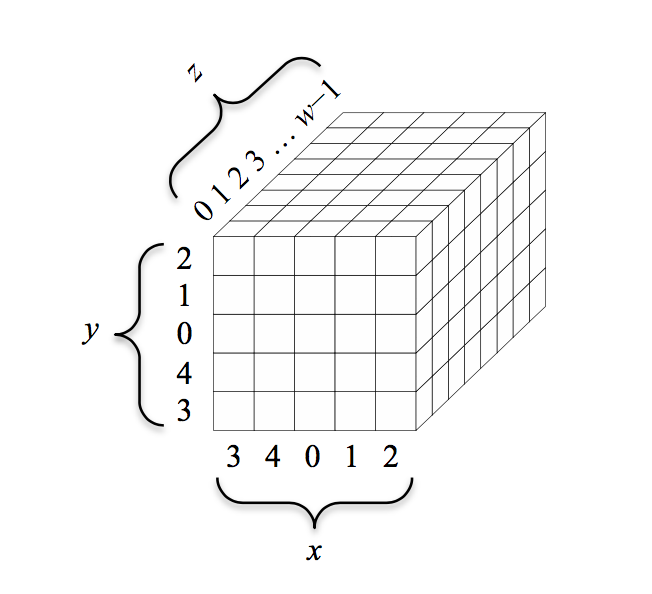
\includegraphics[width=0.55\textwidth]{chapters/pictures/keccak_state.png}
\caption[{Stanje permutacije Keccak-$f[1600]$}]{Stanje permutacije Keccak-$f[1600]$. Preuzeto iz \cite{keccak}}
\label{fig:keccak_stanje}
\end{figure}

Permutacija se sastoji od 24 runde, a svaka runda primenjuje redom pet koraka, $\theta$, $\rho$, $\pi$, $\chi$ i $\iota$, kako je prikazano na slici \ref{fig:keccak_runda}. Svi indeksi u nastavku računaju se po modulu 5, a $\mathrm{rot}(\cdot, k)$ označava cikličko pomeranje trake za $k$ bitova. U nastavku je svaki korak opisan pojedinačno.

\begin{figure}[H]
\centering
\resizebox{0.9\textwidth}{!}{
\begin{tikzpicture}
    \node (sin) [blokdata, minimum width=1.6cm] at (0,0) {$S_{\mathrm{ulaz}}$};
    \node (theta) [blokkripto, minimum width=1.2cm] at (2.2,0) {$\theta$};
    \node (rho) [blokkripto, minimum width=1.2cm] at (3.9,0) {$\rho$};
    \node (pi) [blokkripto, minimum width=1.2cm] at (5.6,0) {$\pi$};
    \node (chi) [blokkripto, minimum width=1.2cm] at (7.3,0) {$\chi$};
    \node (iota) [blokkripto, minimum width=1.2cm] at (9.0,0) {$\iota$};
    \node (sout) [blokrezultat, minimum width=1.6cm] at (11.2,0) {$S_{\mathrm{izlaz}}$};
    \draw [strelica] (sin) -- (theta);
    \draw [strelica] (theta) -- (rho);
    \draw [strelica] (rho) -- (pi);
    \draw [strelica] (pi) -- (chi);
    \draw [strelica] (chi) -- (iota);
    \draw [strelica] (iota) -- (sout);
\end{tikzpicture}
}
\caption{Jedna runda permutacije Keccak-$f[1600]$}
\label{fig:keccak_runda}
\end{figure}

\subsubsection{Korak \texorpdfstring{$\theta$}{theta}}

Korak $\theta$ je jedini koji meša bitove duž $y$-ose i time obezbeđuje difuziju između kolona. Za svako $x$ najpre se izračuna traka parnosti $C_x$, kao XOR svih pet traka sa tim $x$, pa se od parnosti dve susedne ravni formira korekcija $D_x$ i doda svim trakama ravni $x$:
\begin{align}
    C_x &= \bigoplus_{y=0}^{4} A_{x,y}, \qquad D_x = C_{x-1} \oplus \mathrm{rot}(C_{x+1}, 1), \nonumber\\
    A_{x,y} &\gets A_{x,y} \oplus D_x.
    \label{eq:keccak_theta}
\end{align}
Pošto je XOR bitska operacija, $C_x$ nije jedan bit nego cela traka od 64 bita. Njen bit na dubini $z$ jednak je parnosti onih pet bitova koji na toj dubini čine kolonu $(x,z)$. Dimenzija $z$ se pri tome ne meša, računa se 64 nezavisne parnosti, po jedna za svaku dubinu. Jedina operacija u ovom koraku koja uopšte pomera bitove duž $z$-ose jeste rotacija za jedno mesto u izrazu za $D_x$. Sve ostalo se odvija bit po bit, na istoj dubini.
\smallbreak
Ako se izraz (\ref{eq:keccak_theta}) raspiše na nivou pojedinačnog bita, dobija se
\begin{align}
    A_{x,y}[z] \;\gets\;\; & A_{x,y}[z] \nonumber\\[0.4ex]
    &\oplus\; \underbrace{\bigoplus_{y'=0}^{4} A_{x-1,\,y'}[z]}_{\text{parnost kolone } (x-1,\;z)} \nonumber\\[0.4ex]
    &\oplus\; \underbrace{\bigoplus_{y'=0}^{4} A_{x+1,\,y'}[z-1]}_{\text{parnost kolone } (x+1,\;z-1)},
\end{align}
gde $A_{x,y}[z]$ označava bit na dubini $z$ trake $A_{x,y}$.
Svaki izlazni bit zavisi, dakle, od jedanaest ulaznih, od sebe samog i od dve pune kolone. Isto važi i u suprotnom smeru, jer jedan ulazni bit ulazi u jedanaest izlaznih. Otuda brza difuzija, jer promena jednog jedinog bita stanja već posle nekoliko rundi zahvata celo stanje. Delovanje koraka po ravnima prikazano je na slici \ref{fig:keccak_theta}.
\smallbreak
U hardveru $\theta$ nosi najdužu kombinacionu putanju od pet koraka, ali je i ona plitka, jer je parnost XOR sa pet ulaza, koji staje u jedan šestoulazni LUT, pa je ceo korak dubok svega tri nivoa logike, parnosti kolona, korekcije $D_x$ i završnog XOR-a. Nema ni množenja ni tabela u memoriji.

\begin{figure}[H]
\centering
\resizebox{0.40\textwidth}{!}{
{\kvsetup
\begin{tabular}{|c|c|c|c|c|c|}
\hline
\rowcolor{gray!30}
\makebox[1cm]{} & \kv{$x{=}0$} & \kv{$x{=}1$} & \kv{$x{=}2$} & \kv{$x{=}3$} & \kv{$x{=}4$} \\
\hline
\cellcolor{gray!30}\kv{$y{=}0$} & \cellcolor{cyan!30}\kv{$A_{0,0}$} & \cellcolor{green!30}\kv{$A_{1,0}$} & \cellcolor{yellow!30}\kv{$A_{2,0}$} & \kv{$A_{3,0}$} & \kv{$A_{4,0}$} \\
\hline
\cellcolor{gray!30}\kv{$y{=}1$} & \cellcolor{cyan!30}\kv{$A_{0,1}$} & \cellcolor{green!30}\kv{$A_{1,1}$} & \cellcolor{yellow!30}\kv{$A_{2,1}$} & \kv{$A_{3,1}$} & \kv{$A_{4,1}$} \\
\hline
\cellcolor{gray!30}\kv{$y{=}2$} & \cellcolor{cyan!30}\kv{$A_{0,2}$} & \cellcolor{green!30}\kv{$A_{1,2}$} & \cellcolor{yellow!30}\kv{$A_{2,2}$} & \kv{$A_{3,2}$} & \kv{$A_{4,2}$} \\
\hline
\cellcolor{gray!30}\kv{$y{=}3$} & \cellcolor{cyan!30}\kv{$A_{0,3}$} & \cellcolor{green!30}\kv{$A_{1,3}$} & \cellcolor{yellow!30}\kv{$A_{2,3}$} & \kv{$A_{3,3}$} & \kv{$A_{4,3}$} \\
\hline
\cellcolor{gray!30}\kv{$y{=}4$} & \cellcolor{cyan!30}\kv{$A_{0,4}$} & \cellcolor{green!30}\kv{$A_{1,4}$} & \cellcolor{yellow!30}\kv{$A_{2,4}$} & \kv{$A_{3,4}$} & \kv{$A_{4,4}$} \\
\hline
\end{tabular}
}}
\caption{Korak $\theta$ za ravan $x=1$ -- svaka traka ravni (zeleno) sabira se sa trakom parnosti ravni $x=0$ (cijan) i rotiranom trakom parnosti ravni $x=2$ (žuto)}
\label{fig:keccak_theta}
\end{figure}

\subsubsection{Korak \texorpdfstring{$\rho$}{rho}}

Korak $\rho$ ciklično rotira svaku traku za njen fiksni ofset:
\begin{equation}
    A_{x,y} \gets \mathrm{rot}\big(A_{x,y},\, r_{x,y}\big),
\end{equation}
gde su $r_{x,y}$ konstante definisane standardom, date u dodatku \ref{app:keccak}. Rotacija premešta bitove unutar trake (duž $z$-ose stanja), čime difuzija iz koraka $\theta$, koja deluje po kolonama, dobija i treću dimenziju. Delovanje na jednu traku prikazano je na slici \ref{fig:keccak_rho}. U hardveru su ove rotacije fiksne i svode se na preusmeravanje veza, pa ne troše logiku.

\begin{figure}[H]
\centering
\resizebox{0.58\textwidth}{!}{
{\kvsetup
\begin{tabular}{c}
    \begin{tabular}{|c|c|c|c|c|c|c|c|}
    \hline
    \kv{$a_7$} & \kv{$a_6$} & \kv{$a_5$} & \kv{$a_4$} & \kv{$a_3$} & \cellcolor{green!30}\kv{$a_2$} & \cellcolor{green!30}\kv{$a_1$} & \cellcolor{green!30}\kv{$a_0$} \\
    \hline
    \end{tabular}
    \\[2ex]
    $\Big\downarrow\;\mathrm{rot}(\cdot,\,3)$
    \\[2ex]
    \begin{tabular}{|c|c|c|c|c|c|c|c|}
    \hline
    \kv{$a_4$} & \kv{$a_3$} & \cellcolor{green!30}\kv{$a_2$} & \cellcolor{green!30}\kv{$a_1$} & \cellcolor{green!30}\kv{$a_0$} & \kv{$a_7$} & \kv{$a_6$} & \kv{$a_5$} \\
    \hline
    \end{tabular}
\end{tabular}
}}
\caption[Korak $\rho$: ciklična rotacija trake]{Korak $\rho$: ciklična rotacija trake, prikazana na skraćenoj traci od 8 bitova za ofset 3. Tri istaknuta bita prelaze sa desnog kraja na poziciju tri mesta levlje. Bitovi koji izađu sa levog kraja ulaze sa desnog}
\label{fig:keccak_rho}
\end{figure}

\subsubsection{Korak \texorpdfstring{$\pi$}{pi}}

Korak $\pi$ premešta trake na nove pozicije u $5 \times 5$ matrici:
\begin{equation}
    A'_{\,y,\;(2x+3y) \bmod 5} \gets A_{x,y}.
\end{equation}
Dok $\rho$ meša bitove unutar traka, $\pi$ meša same trake između vrsta i kolona, čime se sprečava da se difuzija zadrži u lokalnim šablonima. Preslikavanje svih 25 traka prikazano je na slici \ref{fig:keccak_pi}. Iz izraza za odredište vidi se pravilnost koju slika čini očiglednom. Prvi indeks odredišta je $y$, pa sve trake jedne vrste polaznog stanja završavaju u istoj koloni novog stanja. Korak $\pi$ je, dakle, transpozicija propraćena preslikavanjem $x \mapsto 2x + 3y$ unutar kolone. Traka $A_{0,0}$ jedina ostaje na svom mestu, a duž prve vrste novog stanja poređala se dijagonala polaznog. I ovaj korak je u hardveru besplatan. Kao i ShiftRows transformacija AES algoritma, o kojoj će biti reči u odeljku \ref{subsec:aes_transformacije}, i ovde je reč o čistom preusmeravanju veza.

\begin{figure}[H]
\centering
\resizebox{\textwidth}{!}{
{\kvsetup
\begin{tabular}{c c c}
    \begin{tabular}{|c|c|c|c|c|c|}
    \hline
    \rowcolor{gray!30}
    \makebox[1cm]{} & \kv{$x{=}0$} & \kv{$x{=}1$} & \kv{$x{=}2$} & \kv{$x{=}3$} & \kv{$x{=}4$} \\
    \hline
    \cellcolor{gray!30}\kv{$y{=}0$} & \cellcolor{green!30}\kv{$A_{0,0}$} & \cellcolor{green!30}\kv{$A_{1,0}$} & \cellcolor{green!30}\kv{$A_{2,0}$} & \cellcolor{green!30}\kv{$A_{3,0}$} & \cellcolor{green!30}\kv{$A_{4,0}$} \\
    \hline
    \cellcolor{gray!30}\kv{$y{=}1$} & \cellcolor{yellow!30}\kv{$A_{0,1}$} & \cellcolor{yellow!30}\kv{$A_{1,1}$} & \cellcolor{yellow!30}\kv{$A_{2,1}$} & \cellcolor{yellow!30}\kv{$A_{3,1}$} & \cellcolor{yellow!30}\kv{$A_{4,1}$} \\
    \hline
    \cellcolor{gray!30}\kv{$y{=}2$} & \cellcolor{cyan!30}\kv{$A_{0,2}$} & \cellcolor{cyan!30}\kv{$A_{1,2}$} & \cellcolor{cyan!30}\kv{$A_{2,2}$} & \cellcolor{cyan!30}\kv{$A_{3,2}$} & \cellcolor{cyan!30}\kv{$A_{4,2}$} \\
    \hline
    \cellcolor{gray!30}\kv{$y{=}3$} & \cellcolor{purple!30}\kv{$A_{0,3}$} & \cellcolor{purple!30}\kv{$A_{1,3}$} & \cellcolor{purple!30}\kv{$A_{2,3}$} & \cellcolor{purple!30}\kv{$A_{3,3}$} & \cellcolor{purple!30}\kv{$A_{4,3}$} \\
    \hline
    \cellcolor{gray!30}\kv{$y{=}4$} & \cellcolor{orange!30}\kv{$A_{0,4}$} & \cellcolor{orange!30}\kv{$A_{1,4}$} & \cellcolor{orange!30}\kv{$A_{2,4}$} & \cellcolor{orange!30}\kv{$A_{3,4}$} & \cellcolor{orange!30}\kv{$A_{4,4}$} \\
    \hline
    \end{tabular}
    &
    \raisebox{-16ex}{\Huge $\;\longrightarrow\;$}
    &
    \begin{tabular}{|c|c|c|c|c|c|}
    \hline
    \rowcolor{gray!30}
    \makebox[1cm]{} & \kv{$x{=}0$} & \kv{$x{=}1$} & \kv{$x{=}2$} & \kv{$x{=}3$} & \kv{$x{=}4$} \\
    \hline
    \cellcolor{gray!30}\kv{$y{=}0$} & \cellcolor{green!30}\kv{$A_{0,0}$} & \cellcolor{yellow!30}\kv{$A_{1,1}$} & \cellcolor{cyan!30}\kv{$A_{2,2}$} & \cellcolor{purple!30}\kv{$A_{3,3}$} & \cellcolor{orange!30}\kv{$A_{4,4}$} \\
    \hline
    \cellcolor{gray!30}\kv{$y{=}1$} & \cellcolor{green!30}\kv{$A_{3,0}$} & \cellcolor{yellow!30}\kv{$A_{4,1}$} & \cellcolor{cyan!30}\kv{$A_{0,2}$} & \cellcolor{purple!30}\kv{$A_{1,3}$} & \cellcolor{orange!30}\kv{$A_{2,4}$} \\
    \hline
    \cellcolor{gray!30}\kv{$y{=}2$} & \cellcolor{green!30}\kv{$A_{1,0}$} & \cellcolor{yellow!30}\kv{$A_{2,1}$} & \cellcolor{cyan!30}\kv{$A_{3,2}$} & \cellcolor{purple!30}\kv{$A_{4,3}$} & \cellcolor{orange!30}\kv{$A_{0,4}$} \\
    \hline
    \cellcolor{gray!30}\kv{$y{=}3$} & \cellcolor{green!30}\kv{$A_{4,0}$} & \cellcolor{yellow!30}\kv{$A_{0,1}$} & \cellcolor{cyan!30}\kv{$A_{1,2}$} & \cellcolor{purple!30}\kv{$A_{2,3}$} & \cellcolor{orange!30}\kv{$A_{3,4}$} \\
    \hline
    \cellcolor{gray!30}\kv{$y{=}4$} & \cellcolor{green!30}\kv{$A_{2,0}$} & \cellcolor{yellow!30}\kv{$A_{3,1}$} & \cellcolor{cyan!30}\kv{$A_{4,2}$} & \cellcolor{purple!30}\kv{$A_{0,3}$} & \cellcolor{orange!30}\kv{$A_{1,4}$} \\
    \hline
    \end{tabular}
\end{tabular}
}
}
\caption[Korak $\pi$: preslikavanje svih 25 traka]{Korak $\pi$: preslikavanje svih 25 traka. Levo je polazno, desno novo stanje. U svakoj ćeliji novog stanja upisana je traka koja je na to mesto došla, a boja prati polaznu vrstu $y$}
\label{fig:keccak_pi}
\end{figure}

\subsubsection{Korak \texorpdfstring{$\chi$}{chi}}

Korak $\chi$ je jedina nelinearna operacija permutacije, analogon S-boksa AES algoritma, o kome će biti reči u odeljku \ref{subsec:aes_transformacije}, ali izuzetno jeftin. Deluje po vrstama stanja, dakle za fiksno $y$, tako što se svaka traka sabira sa proizvodom komplementa prve i vrednosti druge naredne trake u istoj vrsti:
\begin{equation}
    A_{x,y} \gets A_{x,y} \oplus \big(\overline{A_{x+1,y}} \wedge A_{x+2,y}\big).
\end{equation}
Operacija je bitska. Logička mreža sa slike \ref{fig:keccak_chi} deluje na svaki od 64 bita trake nezavisno i paralelno, pa se u hardveru sastoji od 1600 identičnih kopija jednog NOT, jednog AND i jednog XOR kola, što je ekvivalent nelinearne supstitucije nad svih 1600 bitova stanja odjednom, bez ijedne memorijske tabele.

\begin{figure}[H]
\centering
\resizebox{0.75\textwidth}{!}{
\begin{tikzpicture}
    \node (a0) [blokdata, minimum width=2.1cm] at (0,0) {$A_{x,y}$};
    \node (a1) [blokdata, minimum width=2.1cm] at (0,-1.3) {$A_{x{+}1,y}$};
    \node (a2) [blokdata, minimum width=2.1cm] at (0,-2.6) {$A_{x{+}2,y}$};
    \node (inv) [circle, draw=black, thick, inner sep=2pt] at (2.7,-1.3) {$\lnot$};
    \node (and) [circle, draw=black, thick, inner sep=2pt] at (4.2,-1.95) {$\wedge$};
    \node (xor) [circle, draw=black, thick, inner sep=2pt] at (5.7,0) {$\oplus$};
    \node (out) [blokrezultat, minimum width=2.3cm] at (7.9,0) {$A'_{x,y}$};
    \draw [strelica] (a1) -- (inv);
    \draw [strelica] (inv) -| (and);
    \draw [strelica] (a2) -| (and);
    \draw [strelica] (a0) -- (xor);
    \draw [strelica] (and) -| (xor);
    \draw [strelica] (xor) -- (out);
\end{tikzpicture}
}
\caption{Korak $\chi$: logika za jednu traku}
\label{fig:keccak_chi}
\end{figure}

\subsubsection{Korak \texorpdfstring{$\iota$}{iota}}

Poslednji korak runde sabira konstantu runde sa jednom jedinom trakom:
\begin{equation}
    A_{0,0} \gets A_{0,0} \oplus RC_i,
\end{equation}
gde je $RC_i$ konstanta runde $i$, definisana standardom (sve 24 vrednosti date su u dodatku \ref{app:keccak}). Bez ovog koraka sve runde bile bi identične, pa bi permutacija imala simetrije koje Oskar može iskoristiti. Konstante, različite u svakoj rundi, tu simetriju narušavaju, a delovanje je prikazano na slici \ref{fig:keccak_iota}.

\begin{figure}[H]
\centering
\begin{tikzpicture}
    \node (a00) [blokdata, minimum width=2.2cm] {$A_{0,0}$};
    \node (xor) [circle, draw=black, thick, right=1.5cm of a00, inner sep=2pt] {$\oplus$};
    \node (rc) [rectangle, rounded corners, draw=black, fill=gray!30, minimum width=2cm, minimum height=0.9cm, above=1cm of xor] {$RC_i$};
    \node (out) [blokrezultat, minimum width=2.2cm, right=1.5cm of xor] {$A'_{0,0}$};
    \draw [strelica] (a00) -- (xor);
    \draw [strelica] (rc) -- (xor);
    \draw [strelica] (xor) -- (out);
\end{tikzpicture}
\caption{Korak $\iota$}
\label{fig:keccak_iota}
\end{figure}
\smallbreak
Sa stanovišta hardverske realizacije, presudno je da se svi koraci svode na bitske operacije XOR, AND, NOT i fiksne rotacije, pri čemu fiksne rotacije u hardveru ne koštaju ništa. Jedna runda je stoga plitka kombinaciona mreža, a cela permutacija se prirodno realizuje iterativno, sa jednom rundom po taktu.

\subsection{Varijante standarda}
\label{subsec:sha3_varijante}

FIPS 202 definiše četiri heš funkcije fiksnog izlaza i dve XOF funkcije, sve nad istom permutacijom Keccak-$f[1600]$, a međusobno različite samo po brzini $r$, kapacitetu $c$ i dužini izlaza, kako je dato u tabeli \ref{tab:sha3_varijante}.

\begin{table}[H]
\caption[Varijante SHA-3 standarda]{Varijante SHA-3 standarda \cite{fips202}}
\centering
\resizebox{0.9\textwidth}{!}{
\begin{tabular}{|c|c|c|c|c|c|}
\hline
\rowcolor{gray!30}
\rsz[2.4cm]{1.2}{Funkcija} & \rsz[1.6cm]{1.2}{$r$ [bit]} & \rsz[1.6cm]{1.2}{$c$ [bit]} & \rsz[2.4cm]{1.2}{Izlaz $d$ [bit]} & \rsz[2.8cm]{1.2}{Kolizije [bit]} & \rsz[2.8cm]{1.2}{Original [bit]} \\
\hline
\rsz[2.2cm]{1.2}{SHA3-224} & \rsz[1cm]{1.2}{1152} & \rsz[1cm]{1.2}{448} & \rsz[1.4cm]{1.2}{224} & \rsz[1.4cm]{1.2}{112} & \rsz[1.4cm]{1.2}{224} \\
\hline
\rsz[2.2cm]{1.2}{SHA3-256} & \rsz[1cm]{1.2}{1088} & \rsz[1cm]{1.2}{512} & \rsz[1.4cm]{1.2}{256} & \rsz[1.4cm]{1.2}{128} & \rsz[1.4cm]{1.2}{256} \\
\hline
\rsz[2.2cm]{1.2}{SHA3-384} & \rsz[1cm]{1.2}{832} & \rsz[1cm]{1.2}{768} & \rsz[1.4cm]{1.2}{384} & \rsz[1.4cm]{1.2}{192} & \rsz[1.4cm]{1.2}{384} \\
\hline
\rsz[2.2cm]{1.2}{SHA3-512} & \rsz[1cm]{1.2}{576} & \rsz[1cm]{1.2}{1024} & \rsz[1.4cm]{1.2}{512} & \rsz[1.4cm]{1.2}{256} & \rsz[1.4cm]{1.2}{512} \\
\hline
\rsz[2.2cm]{1.2}{SHAKE128} & \rsz[1cm]{1.2}{1344} & \rsz[1cm]{1.2}{256} & \rsz[2.2cm]{1.2}{proizvoljan} & \rsz[2.4cm]{1.2}{$\min(d/2,\,128)$} & \rsz[2.4cm]{1.2}{$\min(d,\,128)$} \\
\hline
\rsz[2.2cm]{1.2}{SHAKE256} & \rsz[1cm]{1.2}{1088} & \rsz[1cm]{1.2}{512} & \rsz[2.2cm]{1.2}{proizvoljan} & \rsz[2.4cm]{1.2}{$\min(d/2,\,256)$} & \rsz[2.4cm]{1.2}{$\min(d,\,256)$} \\
\hline
\end{tabular}
}
\label{tab:sha3_varijante}
\end{table}

Činjenica da sve varijante dele istu permutaciju izuzetno je povoljna za hardver, jer je jedno jezgro permutacije dovoljno za ceo standard, a varijanta se bira samo upravljačkom logikom koja određuje koliko se bitova stanja puni, odnosno čita. Uočava se i prirodan kompromis. Varijante sa većim kapacitetom pružaju veću sigurnost, ali obrađuju manje bitova poruke po pozivu permutacije, dakle imaju manju propusnost.

\subsection{Izvedene funkcije: cSHAKE i KMAC}
\label{subsec:kmac}

Nad istom sponge konstrukcijom NIST je standardom SP 800-185 \cite{sp800185} definisao familiju izvedenih funkcija (engl. \textit{derived functions}), od kojih su za ovaj rad značajne cSHAKE i KMAC.
\smallbreak
\textit{cSHAKE} (engl. \textit{customizable SHAKE}) proširuje SHAKE funkcije sa dva dodatna parametra: imenom funkcije $N$, rezervisanim za NIST-ove definicije, i oznakom namene (engl. \textit{customization string}) $S$, kojom korisnik razdvaja različite upotrebe iste funkcije. Parametri se kodiraju u prefiksni blok od jednog ili više celih $r$-bitnih blokova (za ime i oznaku namene iz ovog rada tačno jedan), koji se upija pre same poruke, a sufiks za razdvajanje domena iz tabele \ref{tab:sha3_domeni} menja se u \texttt{00} umesto \texttt{1111} kod SHAKE funkcija, dakle u bajt \texttt{0x04} umesto \texttt{0x1F}.
\smallbreak
Slučaj kada su i $N$ i $S$ prazni standard uređuje posebnim pravilom, a ne kao posledicu konstrukcije. Tada je po definiciji $\mathrm{cSHAKE}(X, L, \texttt{""}, \texttt{""}) = \mathrm{SHAKE}(X, L)$ \cite{sp800185}. To znači da se u tom slučaju prefiksni blok uopšte ne formira i da se koristi SHAKE sufiks \texttt{1111}, dakle bajt \texttt{0x1F}. Bez tog izuzetka cSHAKE sa praznim parametrima ne bi davao isti izlaz kao SHAKE, upravo zato što bi sufiks bio drugačiji.
\smallbreak
Pre same definicije KMAC funkcije potrebne su četiri pomoćne funkcije kodiranja iz standarda \cite{sp800185}. Parametri koji ulaze u konstrukciju dve su vrste: brojevi (dužine) i stringovi (ime funkcije, oznaka namene, ključ), a ove četiri funkcije ih prevode u zapis iz koga se svaki sastavni deo može jednoznačno pročitati. Time se sprečava da dva različita skupa parametara daju isti ulazni niz. Sve četiri sažeto su date u tabeli \ref{tab:sp800185_kodiranja}.

\begin{table}[H]
\caption[Pomoćne funkcije kodiranja iz standarda SP 800-185]{Pomoćne funkcije kodiranja iz standarda SP 800-185 \cite{sp800185}}
\centering
\resizebox{\textwidth}{!}{
\begin{tabular}{|c|c|c|}
\hline
\rowcolor{gray!30}
\rsz[4cm]{1.2}{Funkcija} & \rsz[7cm]{1.2}{Rezultat} & \rsz[7cm]{1.2}{Uloga} \\
\hline
\rsz[4.4cm]{1.2}{$\mathrm{left\_encode}(x)$} & \makecell{\rsz[6.6cm]{1.2}{dužina zapisa, pa sam broj $x$} \\ \rsz[6.6cm]{1.2}{(brojač dužine ispred)}} & \rsz[7cm]{1.2}{dužina koja prethodi podatku} \\
\hline
\rsz[4.4cm]{1.2}{$\mathrm{right\_encode}(x)$} & \makecell{\rsz[6.6cm]{1.2}{broj $x$, pa dužina zapisa} \\ \rsz[6.6cm]{1.2}{(brojač dužine iza)}} & \rsz[7cm]{1.2}{dužina koja sledi iza podatka} \\
\hline
\rsz[4.4cm]{1.2}{$\mathrm{encode\_string}(S)$} & \rsz[6.6cm]{1.2}{$\mathrm{left\_encode}(\mathrm{len}(S)) \,\|\, S$} & \rsz[7cm]{1.2}{string kome prethodi dužina} \\
\hline
\rsz[4.4cm]{1.2}{$\mathrm{bytepad}(X, w)$} & \makecell{\rsz[6.6cm]{1.2}{$\mathrm{left\_encode}(w) \,\|\, X$, dopunjeno} \\ \rsz[6.6cm]{1.2}{nulama do umnoška $w$ bajtova}} & \rsz[7cm]{1.2}{poravnanje na granicu bloka} \\
\hline
\end{tabular}
}
\label{tab:sp800185_kodiranja}
\end{table}

Dve varijante zapisa dužine postoje zbog dva različita mesta na kojima zapis stoji. Kada dužina prethodi podatku, čitalac je pročita pa zna koliko bajtova posle nje da uzme. Tako rade prefiksni blok i blok ključa, iza kojih sledi još sadržaja. Kodirana dužina izlaza, međutim, stoji na samom kraju ulaznog niza, iza poruke čija dužina unapred nije poznata, pa se do nje dolazi čitanjem sa kraja. Poslednji bajt kaže koliko bajtova broja stoji ispred njega, pa ona zato koristi $\mathrm{right\_encode}$.
\smallbreak
\textit{KMAC} (engl. \textit{Keccak Message Authentication Code}) je funkcija sa tajnim ključem izgrađena nad cSHAKE funkcijom sa imenom $N = \texttt{"KMAC"}$:
\begin{align}
    \mathrm{KMAC}[K, X, L, S] = \mathrm{cSHAKE}\big(
        &\mathrm{bytepad}(\mathrm{encode\_string}(K),\, r/8) \nonumber\\
        &\quad {}\,\|\, X \,\|\, \mathrm{right\_encode}(L), \nonumber\\
        &L,\; \texttt{"KMAC"},\; S\big),
    \label{eq:kmac}
\end{align}
gde se ključ $K$ kodira i dopuni u ceo blok koji se upija pre poruke $X$, a $\mathrm{right\_encode}(L)$ na kraj poruke dodaje kodiranu dužinu izlaza $L$ (varijanta KMACXOF, sa $\mathrm{right\_encode}(0)$, daje izlaz proizvoljne dužine u XOF režimu).
\smallbreak
Postavlja se pitanje zašto je posebna konstrukcija uopšte potrebna, kada sunđer nema svojstvo produženja poruke (odeljak \ref{subsec:sponge_sigurnost}), pa naivni oblik $H(K \,\|\, X)$ nad SHA-3 funkcijom nije ugrožen napadom koji kod Merkle--Damgardove klase nameće HMAC. KMAC ipak donosi tri svojstva koja taj oblik nema. Prva je kodiranje ključa sa dužinom upisanom ispred njega, čime granica ključa postaje deo samog niza, pa dva različita para ključa i poruke nikada ne daju isti ulaz. Druga je razdvajanje domena kroz ime $N$ i oznaku namene $S$, čime se isti ključ bezbedno koristi za više namena. Treća je kodirana dužina izlaza, čime skraćen izlaz nije prefiks dužeg. Rezultat je standardizovana pseudoslučajna funkcija (engl. \textit{pseudorandom function}, PRF) čija sigurnost počiva neposredno na kapacitetu sponge konstrukcije, odobrena i kao MAC i kao funkcija za izvođenje ključeva, i sve to jednim pozivom heš funkcije, bez dva ulančana poziva koja traži HMAC.
\smallbreak
Iako izraz (\ref{eq:kmac}) deluje glomazno, on ne uvodi nikakvo novo izračunavanje. Sve što opisuje jeste redosled kojim se polja nadovezuju u ulazni niz pre upijanja. Kako sastavljeni niz izgleda prikazuje slika \ref{fig:kmac_okvir}. Bitno je uočiti da su prva dva polja celi $r$-bitni blokovi. Prefiksni blok nosi ime funkcije i oznaku namene, a blok ključa je dopunjen funkcijom $\mathrm{bytepad}$ do granice bloka. Tek posle njih dolazi sama poruka, pa kodirana dužina izlaza, i na kraju dopuna iz odeljka \ref{subsec:sha3_dopuna} sa sufiksom \texttt{00}, jer je reč o cSHAKE funkciji.

\begin{figure}[H]
\centering
\setlength{\tabcolsep}{8pt}
\renewcommand{\arraystretch}{1.6}
\resizebox{\textwidth}{!}{
\begin{tabular}{|c|c|c|c|c|}
\multicolumn{1}{c}{ceo blok od $r$ bitova} & \multicolumn{1}{c}{ceo blok od $r$ bitova} & \multicolumn{3}{c}{} \\
\hline
\cellcolor{cyan!30}prefiksni blok $(N, S)$ & \cellcolor{purple!30}blok ključa $K$ & \cellcolor{green!30}poruka $X$ & \cellcolor{yellow!30}$\mathrm{right\_encode}(L)$ & \cellcolor{gray!30}dopuna \\
\hline
\end{tabular}
}
\caption[Uokvirivanje ulaznog niza KMAC funkcije]{Uokvirivanje ulaznog niza KMAC funkcije pre upijanja}
\label{fig:kmac_okvir}
\end{figure}

\begin{example}
\label{ex:kmac_bajtovi}
U ulozi koju KMAC256 ima u ovom radu, u izvođenju ključeva, ulogu ključa $K$ ima so (engl. \textit{salt}) od 32 bajta, poruka $X$ nosi zajedničku tajnu i kontekst razmene, ovde 72 bajta tajne i 40 bajtova konteksta, ukupno 112, oznaka namene $S$ je \texttt{"KDF"}, kako za ovu ulogu propisuje SP 800-56C \cite{sp80056c}, a dužina izlaza $L = 256$ bitova odgovara ključu za AES-256 (raspodela parametara data je u tabeli \ref{tab:kmac_uloge}). Brzina upijanja je $r/8 = 136$ bajtova, pa je $\mathrm{left\_encode}(136) = \texttt{01 88}$, i tim parom počinju oba uokvirena bloka:
\begin{center}
\small
\setlength{\tabcolsep}{6pt}
\renewcommand{\arraystretch}{1.3}
\begin{tabular}{|l|l|l|}
\hline
\rowcolor{gray!30}
Bajtovi & Zapis & Značenje \\
\hline
\cellcolor{cyan!30}\texttt{01 88} & $\mathrm{left\_encode}(136)$ & brzina upijanja $r/8$ \\
\hline
\cellcolor{cyan!30}\texttt{01 20} & $\mathrm{left\_encode}(32)$ & dužina imena, $4 \cdot 8$ bitova \\
\hline
\cellcolor{cyan!30}\texttt{4B 4D 41 43} & \texttt{"KMAC"} u ASCII zapisu & ime funkcije $N$ \\
\hline
\cellcolor{cyan!30}\texttt{01 18} & $\mathrm{left\_encode}(24)$ & dužina oznake, $3 \cdot 8$ bitova \\
\hline
\cellcolor{cyan!30}\texttt{4B 44 46} & \texttt{"KDF"} u ASCII zapisu & oznaka namene $S$ \\
\hline
\cellcolor{gray!30}\texttt{00} $\times\,123$ & dopuna nulama & do granice prvog bloka \\
\hline
\cellcolor{purple!30}\texttt{01 88} & $\mathrm{left\_encode}(136)$ & brzina upijanja $r/8$ \\
\hline
\cellcolor{purple!30}\texttt{02 01 00} & $\mathrm{left\_encode}(256)$ & dužina ključa, $32 \cdot 8$ bitova \\
\hline
\cellcolor{purple!30}$K$, 32 bajta & --- & so, u ulozi ključa \\
\hline
\cellcolor{gray!30}\texttt{00} $\times\,99$ & dopuna nulama & do granice drugog bloka \\
\hline
\cellcolor{green!30}$X$, 112 bajtova & --- & zajednička tajna i kontekst razmene \\
\hline
\cellcolor{yellow!30}\texttt{01 00 02} & $\mathrm{right\_encode}(256)$ & dužina izlaza $L$ \\
\hline
\cellcolor{gray!30}\texttt{04 00 \dots\ 00 80} & sufiks i dopuna & do granice trećeg bloka \\
\hline
\end{tabular}
\end{center}
Dužine stringova izražene su u bitovima, ne u bajtovima, pa ime od četiri znaka daje \texttt{0x20}, a so od 32 bajta vrednost 256, koja se više ne smešta u jedan bajt. U ovom primeru se, sasvim nezavisno od toga, i za dužinu izlaza slučajno bira istih 256 bitova, a mogla je biti i drugačija. Baš zato što je broj isti, na njegova dva zapisa vidi se razlika iz tabele \ref{tab:sp800185_kodiranja}. Zapis \texttt{02 01 00} u bloku ključa čita se unapred, sa brojem bajtova ispred, a \texttt{01 00 02} na kraju niza unazad, sa brojem bajtova iza.
\end{example}

Primer pokazuje i donju granicu cene. Prefiksni blok i blok ključa su celi blokovi bez obzira na to koliko su $N$, $S$ i $K$ kratki, a poruka sa kodiranom dužinom izlaza i završnom dopunom traži bar još jedan, pa KMAC nikada ne košta manje od tri poziva permutacije, ni kada su svi parametri prazni. Kod kratkih ulaza, kakvi se u izvođenju ključeva i javljaju, dva od ta tri bloka nose samo okvir. Isti raspored donosi i pogodnost. Poruka $X$ uvek počinje na poznatoj granici bloka, kod KMAC256 posle tačno 272 bajta okvira, pa strana koja ulazni niz sastavlja upisuje unapred poznate bajtove na unapred poznata mesta i ne mora da prati pomeraj unutar bloka.
\smallbreak
Raspodela parametara iz primera \ref{ex:kmac_bajtovi} upravo je ona koju KMAC ima u hibridnom sistemu iz odeljka \ref{sec:hibridni_sistem}, a to je izvođenje ključeva po jednokoračnoj KDF šemi iz NIST preporuke SP 800-56C \cite{sp80056c}. Ona nije ista kao pri upotrebi za autentifikaciju poruka, a razliku uporedno prikazuje tabela \ref{tab:kmac_uloge}. Suština je u tome što se tajnost seli iz ključa u poruku. Zajednička tajna $Z$ dobijena ECDH razmenom ulazi u poruku $X$, nadovezana sa fiksnim kontekstom razmene (engl. \textit{FixedInfo}), koji obuhvata identitete strana i oznaku protokola, dok je ključ $K$ so, koja po standardu sme biti i unapred dogovorena javna vrednost. Oznaku namene $S$ standard pritom fiksira na vrednost \texttt{"KDF"}, čime je upotreba KMAC-a za izvođenje ključeva razdvojena od svih ostalih upotreba iste funkcije. Ključ sesije i inicijalne vrednosti seku se iz jednog izlaza tražene dužine, a njihov kontekst nosi FixedInfo.

\begin{table}[H]
\caption{Uloge parametara KMAC funkcije: autentifikacija poruka naspram izvođenja ključeva}
\centering
\resizebox{\textwidth}{!}{
\begin{tabular}{|c|c|c|}
\hline
\rowcolor{gray!30}
\rsz[3.4cm]{1.2}{Parametar} & \rsz[6.6cm]{1.2}{KMAC kao MAC} & \rsz[7.4cm]{1.2}{KMAC kao KDF (SP 800-56C)} \\
\hline
\rsz[3cm]{1.2}{ključ $K$} & \rsz[6.2cm]{1.2}{tajni ključ koji strane dele} & \rsz[7cm]{1.2}{so, sme biti i javna vrednost} \\
\hline
\rsz[3cm]{1.2}{poruka $X$} & \rsz[6.2cm]{1.2}{podatak koji se autentifikuje} & \rsz[7cm]{1.2}{$Z \,\|\, \mathrm{FixedInfo}$, tajna je u $Z$} \\
\hline
\rsz[3cm]{1.2}{oznaka $S$} & \rsz[6.2cm]{1.2}{razdvajanje namena istog ključa} & \rsz[7cm]{1.2}{standard je fiksira na \texttt{"KDF"}} \\
\hline
\rsz[3cm]{1.2}{izlaz} & \rsz[6.2cm]{1.2}{autentifikaciona oznaka} & \rsz[7cm]{1.2}{ključni materijal} \\
\hline
\end{tabular}
}
\label{tab:kmac_uloge}
\end{table}

U radu je korišćen KMAC256. Ovim izborom ceo lanac pokriven je NIST standardima: uspostavljanje zajedničke tajne po SP 800-56A \cite{sp80056a}, izvođenje ključeva po SP 800-56C \cite{sp80056c}, a zaštita saobraćaja po SP 800-38D \cite{sp80038d}.
\smallbreak
Celokupno KMAC uokvirivanje, dakle prefiksni blok, blok ključa i kodirana dužina izlaza, jeste čisto formatiranje ulaznog niza, jer nijedan od tih koraka ne dira permutaciju niti stanje sunđera. Za KMAC je zato dovoljna svaka realizacija cSHAKE funkcije. Kako je to iskorišćeno u akceleratoru opisano je u odeljku \ref{subsec:hw_sha3_kmac}.

\section{AES-GCM}
\label{sec:aes_gcm}

Treću komponentu sistema čini AES u GCM režimu rada, algoritam za simetrično šifrovanje kojim se štiti korisnički saobraćaj. U ovom odeljku najpre je opisan sam AES algoritam, njegova arhitektura, transformacije u rundi i ekspanzija ključa, a zatim GCM režim koji od blok šifre gradi autentifikovano šifrovanje. Detaljna analiza AES algoritma, sa kompletnim matematičkim osnovama i izvođenjima nad poljem $\mathrm{GF}(2^8)$, data je u \cite{gavrilovic_diplomski}.
\smallbreak
Izlaganje prati notaciju standarda \cite{fips197, sp80038d} uz jedno odstupanje. Otvoreni tekst, šifrat, autentifikaciona oznaka i pridruženi podaci (engl. \textit{Additional Authenticated Data}) označeni su sa $\mathrm{PT}$, $\mathrm{CT}$, $\mathrm{ICV}$ i $\mathrm{AAD}$, umesto sa $P$, $C$, $T$ i $A$. Razlog je dvostruk. Takve oznake prate uobičajenu terminologiju mrežnih protokola, a simboli $T$ i $A$ su već zauzeti: $T$ za T-tabele u odeljku \ref{subsec:aes_ttabele}, a $A$ za stanje Keccak permutacije i operande množenja.

\subsection{Nastanak standarda}
\label{subsec:aes_istorijat}

NIST je 1997. godine raspisao javni konkurs za novi standard šifrovanja, kao zamenu za zastareli DES čija je dužina ključa od 56 bitova postala nedovoljna pred rastućom računarskom snagom. Nakon dve runde svetske evaluacije, u kojima su kandidati ocenjivani po sigurnosti, brzini u softveru i hardveru i jednostavnosti realizacije, za pobednika je 2000. godine proglašen algoritam Rijndael belgijskih kriptografa Joana Daemena i Vincenta Rijmena \cite{daemen_rijndael}. Standardizovana verzija, objavljena 2001. godine kao FIPS 197 \cite{fips197}, sužava fleksibilnost izvornog algoritma. Dužina bloka fiksirana je na 128 bitova, a dozvoljene dužine ključa su 128, 192 i 256 bitova, po kojima varijante nose nazive AES-128, AES-192 i AES-256.

\subsection{Arhitektura algoritma}
\label{subsec:aes_arhitektura}

AES obrađuje blok od 128 bitova predstavljen kao matrica $4 \times 4$ bajtova, koja se naziva matrica stanja (engl. \textit{state}). Bajtovi ulaznog bloka pune matricu po kolonama, a svaka transformacija algoritma ažurira stanje novim vrednostima. Broj kolona matrice stanja označava se sa $N_b$ i za AES iznosi $N_b = 128/32 = 4$. Raspored bajtova u matrici prikazan je na slici \ref{fig:aes_matrica_stanja}.

\begin{figure}[H]
\centering
\resizebox{0.30\textwidth}{!}{
{\kvsetup
\begin{tabular}{|c|c|c|c|}
\hline
\kv{$s_{0,0}$} & \kv{$s_{0,1}$} & \kv{$s_{0,2}$} & \kv{$s_{0,3}$} \\
\hline
\kv{$s_{1,0}$} & \kv{$s_{1,1}$} & \kv{$s_{1,2}$} & \kv{$s_{1,3}$} \\
\hline
\kv{$s_{2,0}$} & \kv{$s_{2,1}$} & \kv{$s_{2,2}$} & \kv{$s_{2,3}$} \\
\hline
\kv{$s_{3,0}$} & \kv{$s_{3,1}$} & \kv{$s_{3,2}$} & \kv{$s_{3,3}$} \\
\hline
\end{tabular}
}}
\caption{Matrica stanja AES algoritma}
\label{fig:aes_matrica_stanja}
\end{figure}

Svaki bajt matrice stanja tumači se kao element polja $\mathrm{GF}(2^8)$ sa redukcionim polinomom:
\begin{equation}
    m(x) = x^8 + x^4 + x^3 + x + 1,
    \label{eq:aes_polinom}
\end{equation}
pa su sve operacije nad bajtovima zapravo operacije u tom polju. Sabiranje je XOR, a množenje se izvodi po modulu $m(x)$. Analogno matrici stanja, ključ se predstavlja matricom od $N_k$ kolona, gde je $N_k$ dužina ključa podeljena sa 32. Broj rundi $N_r$ zavisi od dužine ključa, kako je prikazano u tabeli \ref{tab:aes_varijante}.

\begin{table}[H]
\caption[Varijante AES algoritma]{Varijante AES algoritma \cite{fips197}}
\centering
\resizebox{0.75\textwidth}{!}{
\begin{tabular}{|c|c|c|c|}
\hline
\rowcolor{gray!30}
\rsz[2.6cm]{1.2}{Varijanta} & \rsz[4.2cm]{1.2}{Dužina ključa [bit]} & \rsz[1.2cm]{1.2}{$N_k$} & \rsz[1.2cm]{1.2}{$N_r$} \\
\hline
\rsz[2.2cm]{1.2}{AES-128} & \rsz[1.4cm]{1.2}{128} & \rsz[0.8cm]{1.2}{4} & \rsz[0.8cm]{1.2}{10} \\
\hline
\rsz[2.2cm]{1.2}{AES-192} & \rsz[1.4cm]{1.2}{192} & \rsz[0.8cm]{1.2}{6} & \rsz[0.8cm]{1.2}{12} \\
\hline
\rsz[2.2cm]{1.2}{AES-256} & \rsz[1.4cm]{1.2}{256} & \rsz[0.8cm]{1.2}{8} & \rsz[0.8cm]{1.2}{14} \\
\hline
\end{tabular}
}
\label{tab:aes_varijante}
\end{table}

U ovom radu korišćen je AES-256.

\subsection{Tok šifrovanja}
\label{subsec:aes_tok}

Šifrovanje počinje početnom operacijom AddRoundKey, kojom se ulazni blok sabira sa prvim ključem runde operacijom XOR. Zatim sledi $N_r$ rundi, od kojih svaka primenjuje redom četiri transformacije: SubBytes, ShiftRows, MixColumns i AddRoundKey, s tim što se u poslednjoj rundi transformacija MixColumns izostavlja. Svaka runda koristi svoj ključ, dobijen postupkom ekspanzije ključa opisanim u odeljku \ref{subsec:aes_ekspanzija}.
\smallbreak
Svaka od četiri transformacije ima jasno odvojenu ulogu, a raspoređene su po klasičnoj podeli na konfuziju i difuziju:
\begin{itemize}[itemsep=2pt]
    \item SubBytes je nosilac konfuzije i jedina nelinearna operacija u algoritmu. Bez nje bi ceo AES bio linearno preslikavanje, pa i trivijalno rešiv.
    \item ShiftRows i MixColumns zajedno čine linearni sloj, zadužen za difuziju. MixColumns meša četiri bajta unutar kolone, dok ShiftRows ne kombinuje nijedan bajt sa drugim, nego ih samo premešta tako da bajtovi jedne vrste završe u različitim kolonama.
    \item AddRoundKey unosi tajni materijal ključa u stanje. I ona je linearna operacija i sama ne doprinosi ni konfuziji ni difuziji. Njena je uloga da nelinearnost naredne runde ima na šta da deluje.
\end{itemize}
Podela posla unutar linearnog sloja objašnjava zašto su potrebne obe transformacije. MixColumns sam po sebi nikada ne bi izašao iz granica jedne kolone, a ShiftRows sam po sebi ne stvara nikakvu zavisnost među bajtovima. Tek zato što ShiftRows prethodno razmesti bajtove među kolone, MixColumns u narednoj rundi meša bajtove koji su prvobitno pripadali različitim kolonama. Posledica je da već posle dve runde svaki bajt stanja zavisi od svih šesnaest bajtova ulaza, a ponavljanjem kroz sve runde svaki bit izlaza postaje složena funkcija svih bitova ulaza i svih bitova ključa.
Grafički prikaz celokupnog toka dat je na slici \ref{fig:aes_tok_enkripcije}, dok slika \ref{fig:aes_runda} prikazuje delovanje transformacija jedne runde na matricu stanja.

\begin{figure}[H]
\centering
\resizebox{0.72\textwidth}{!}{
\begin{tikzpicture}[node distance=0.45cm]
    \node (in) [blokdata, minimum width=3.4cm] {ulazni tekst};
    \node (ark0) [blokkripto, minimum width=3.4cm, below=0.8cm of in] {AddRoundKey};
    \node (sb) [blokkripto, minimum width=3.4cm, below=1.2cm of ark0] {SubBytes};
    \node (sr) [blokkripto, minimum width=3.4cm, below=of sb] {ShiftRows};
    \node (mc) [blokkripto, minimum width=3.4cm, below=of sr] {MixColumns};
    \node (ark1) [blokkripto, minimum width=3.4cm, below=of mc] {AddRoundKey};
    \node (runda) [draw=black, dashed, thick, inner sep=0.3cm, fit=(sb)(ark1)] {};
    \node [left=0.4cm of runda, align=right] {runda,\\ ponavlja se\\ $N_r - 1$ puta};
    \node (sb2) [blokkripto, minimum width=3.4cm, below=1.5cm of ark1] {SubBytes};
    \node (sr2) [blokkripto, minimum width=3.4cm, below=of sb2] {ShiftRows};
    \node (ark2) [blokkripto, minimum width=3.4cm, below=of sr2] {AddRoundKey};
    \node (finalr) [draw=black, dashed, thick, inner sep=0.3cm, fit=(sb2)(ark2)] {};
    \node [left=0.4cm of finalr, align=right] {poslednja runda\\ (bez MixColumns)};
    \node (out) [blokrezultat, minimum width=3.4cm, below=1.2cm of ark2] {šifrat};
    \draw [strelica] (in) -- (ark0);
    \draw [strelica] (ark0) -- (sb);
    \draw [strelica] (sb) -- (sr);
    \draw [strelica] (sr) -- (mc);
    \draw [strelica] (mc) -- (ark1);
    \draw [strelica] (ark1) -- (sb2);
    \draw [strelica] (sb2) -- (sr2);
    \draw [strelica] (sr2) -- (ark2);
    \draw [strelica] (ark2) -- (out);
    % ekspander kljuca
    \node (kljuc) [blokdata, minimum width=2.6cm, right=3.2cm of in] {ključ};
    \node (ke) [rectangle, rounded corners, draw=black, fill=gray!30, minimum width=2.8cm, minimum height=1.2cm, below=1.6cm of kljuc, align=center] {ekspander\\ ključa};
    \draw [strelica] (kljuc) -- (ke);
    \draw [strelica] (ke) |- node[above, pos=0.8, font=\small] {ključ runde $0$} (ark0.east);
    \draw [strelica] (ke) |- node[above, pos=0.8, font=\small] {ključ runde $i$} (ark1.east);
    \draw [strelica] (ke) |- node[above, pos=0.8, font=\small] {ključ runde $N_r$} (ark2.east);
\end{tikzpicture}
}
\caption{Koraci u AES šifrovanju}
\label{fig:aes_tok_enkripcije}
\end{figure}

\begin{figure}[H]
    \centering
    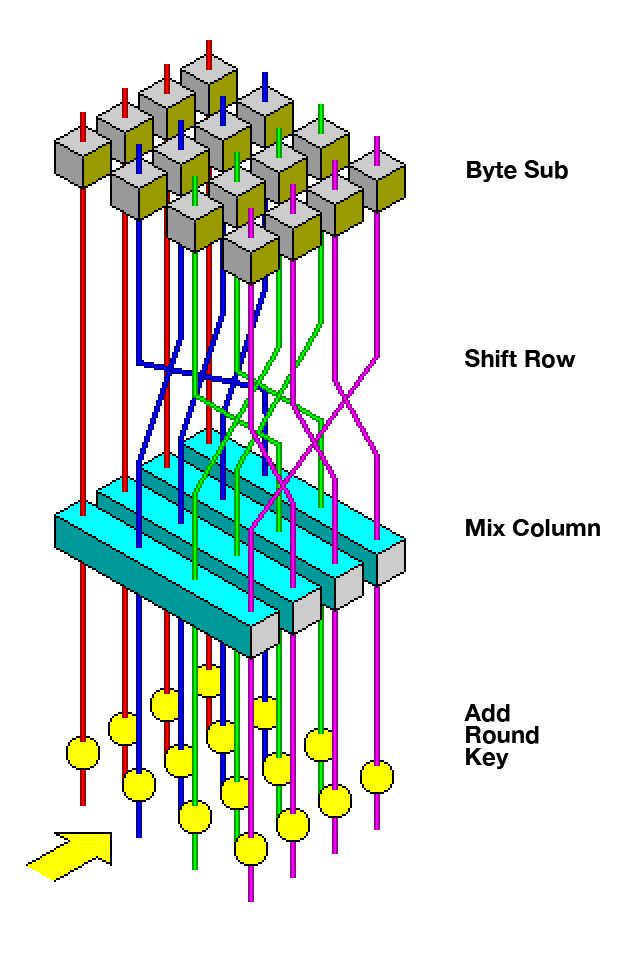
\includegraphics[width=0.45\columnwidth]{chapters/pictures/AES_(Rijndael)_Round_Function.png}
    \caption[Prikaz jedne runde AES šifrovanja]{Prikaz jedne runde AES šifrovanja. Preuzeto iz \cite{savard_aes_round}.}
    \label{fig:aes_runda}
\end{figure}

\subsection{Transformacije u rundi}
\label{subsec:aes_transformacije}

\subsubsection{SubBytes}

SubBytes zamenjuje svaki bajt matrice stanja vrednošću iz supstitucione tabele, S-boksa. Ta tabela nije proizvoljna, već je definisana kompozicijom dve operacije nad bajtom $b$:
\begin{enumerate}[itemsep=2pt]
    \item multiplikativna inverzija u polju $\mathrm{GF}(2^8)$ -- $b \mapsto b^{-1}$, uz dogovor $0 \mapsto 0$;
    \item afina transformacija nad bitovima rezultata:
    \begin{equation}
        b'_i = b_i \oplus b_{(i+4) \bmod 8} \oplus b_{(i+5) \bmod 8} \oplus b_{(i+6) \bmod 8} \oplus b_{(i+7) \bmod 8} \oplus c_i,
        \label{eq:sbox_afina}
    \end{equation}
    gde je $c = \{63\} = 01100011_2$.
\end{enumerate}
Inverzija u polju obezbeđuje visoku nelinearnost i otpornost na diferencijalnu i linearnu kriptoanalizu, dok afina transformacija otklanja fiksne tačke. U realizacijama se S-boks najčešće ostvaruje kao tabela od 256 vrednosti, memorijska ili kombinaciona, mada je moguće i direktno izračunavanje inverzije dekompozicijom polja, što je izbor koji neposredno utiče na površinu i kritičnu putanju hardvera. Transformacija deluje na svaki bajt nezavisno, pa se matrica stanja preslikava element po element, kako prikazuje slika \ref{fig:sbox_pristup}: gornja četiri bita bajta biraju vrstu, a donja četiri kolonu S-boksa. Na slici je istaknut bajt $\{53\}$, koji se preslikava u $\{ED\}$. Kompletna tabela S-boksa data je u dodatku \ref{app:aes_tabele}.

\begin{figure}[H]
\centering
\resizebox{\textwidth}{!}{
\begin{tikzpicture}
    \node (stanje) [inner sep=0pt] {%
    \begin{tabular}{|c|c|c|c|}
    \hline
    \rsz{1.3}{$s_{0,0}$} & \rsz{1.3}{$s_{0,1}$} & \rsz{1.3}{$s_{0,2}$} & \rsz{1.3}{$s_{0,3}$} \\ \hline
    \rsz{1.3}{$s_{1,0}$} & \cellcolor{green!30}\rsz{1.3}{$\{53\}$} & \rsz{1.3}{$s_{1,2}$} & \rsz{1.3}{$s_{1,3}$} \\ \hline
    \rsz{1.3}{$s_{2,0}$} & \rsz{1.3}{$s_{2,1}$} & \rsz{1.3}{$s_{2,2}$} & \rsz{1.3}{$s_{2,3}$} \\ \hline
    \rsz{1.3}{$s_{3,0}$} & \rsz{1.3}{$s_{3,1}$} & \rsz{1.3}{$s_{3,2}$} & \rsz{1.3}{$s_{3,3}$} \\ \hline
    \end{tabular}};
    \node (sbox) [blokkripto, right=1.6cm of stanje, minimum width=3.6cm, minimum height=3cm, align=center, font=\Large] {S-boks\\ $16 \times 16$\\ vrsta $\{5\}$, kolona $\{3\}$};
    \node (novo) [right=1.6cm of sbox, inner sep=0pt] {%
    \begin{tabular}{|c|c|c|c|}
    \hline
    \rsz{1.3}{$s'_{0,0}$} & \rsz{1.3}{$s'_{0,1}$} & \rsz{1.3}{$s'_{0,2}$} & \rsz{1.3}{$s'_{0,3}$} \\ \hline
    \rsz{1.3}{$s'_{1,0}$} & \cellcolor{purple!30}\rsz{1.3}{$\{ED\}$} & \rsz{1.3}{$s'_{1,2}$} & \rsz{1.3}{$s'_{1,3}$} \\ \hline
    \rsz{1.3}{$s'_{2,0}$} & \rsz{1.3}{$s'_{2,1}$} & \rsz{1.3}{$s'_{2,2}$} & \rsz{1.3}{$s'_{2,3}$} \\ \hline
    \rsz{1.3}{$s'_{3,0}$} & \rsz{1.3}{$s'_{3,1}$} & \rsz{1.3}{$s'_{3,2}$} & \rsz{1.3}{$s'_{3,3}$} \\ \hline
    \end{tabular}};
    \draw [strelica] (stanje) -- (sbox);
    \draw [strelica] (sbox) -- (novo);
\end{tikzpicture}
}
\caption{SubBytes transformacija na primeru bajta $\{53\} \mapsto \{ED\}$}
\label{fig:sbox_pristup}
\end{figure}

\subsubsection{ShiftRows}

ShiftRows ciklično pomera vrste matrice stanja ulevo. Vrsta $r$ pomera se za $r$ mesta, dakle nulta vrsta ostaje nepromenjena. Transformacija je prikazana na slici \ref{fig:shiftrows}. Kolone polazne matrice označene su bojama, pa se u rezultatu jasno vidi za koliko je mesta svaka vrsta pomerena.

\begin{figure}[H]
\centering
\resizebox{0.80\textwidth}{!}{
{\kvsetup
\begin{tabular}{c c c}
    \begin{tabular}[c]{|c|c|c|c|}
    \hline
    \cellcolor{green!30}\kv{$s_{0,0}$} & \cellcolor{cyan!30}\kv{$s_{0,1}$} & \cellcolor{yellow!30}\kv{$s_{0,2}$} & \cellcolor{purple!30}\kv{$s_{0,3}$} \\ \hline
    \cellcolor{green!30}\kv{$s_{1,0}$} & \cellcolor{cyan!30}\kv{$s_{1,1}$} & \cellcolor{yellow!30}\kv{$s_{1,2}$} & \cellcolor{purple!30}\kv{$s_{1,3}$} \\ \hline
    \cellcolor{green!30}\kv{$s_{2,0}$} & \cellcolor{cyan!30}\kv{$s_{2,1}$} & \cellcolor{yellow!30}\kv{$s_{2,2}$} & \cellcolor{purple!30}\kv{$s_{2,3}$} \\ \hline
    \cellcolor{green!30}\kv{$s_{3,0}$} & \cellcolor{cyan!30}\kv{$s_{3,1}$} & \cellcolor{yellow!30}\kv{$s_{3,2}$} & \cellcolor{purple!30}\kv{$s_{3,3}$} \\ \hline
    \end{tabular}
    &
    {\Huge $\longrightarrow$}
    &
    \begin{tabular}[c]{|c|c|c|c|}
    \hline
    \cellcolor{green!30}\kv{$s_{0,0}$} & \cellcolor{cyan!30}\kv{$s_{0,1}$} & \cellcolor{yellow!30}\kv{$s_{0,2}$} & \cellcolor{purple!30}\kv{$s_{0,3}$} \\ \hline
    \cellcolor{cyan!30}\kv{$s_{1,1}$} & \cellcolor{yellow!30}\kv{$s_{1,2}$} & \cellcolor{purple!30}\kv{$s_{1,3}$} & \cellcolor{green!30}\kv{$s_{1,0}$} \\ \hline
    \cellcolor{yellow!30}\kv{$s_{2,2}$} & \cellcolor{purple!30}\kv{$s_{2,3}$} & \cellcolor{green!30}\kv{$s_{2,0}$} & \cellcolor{cyan!30}\kv{$s_{2,1}$} \\ \hline
    \cellcolor{purple!30}\kv{$s_{3,3}$} & \cellcolor{green!30}\kv{$s_{3,0}$} & \cellcolor{cyan!30}\kv{$s_{3,1}$} & \cellcolor{yellow!30}\kv{$s_{3,2}$} \\ \hline
    \end{tabular}
\end{tabular}
}}
\caption{ShiftRows transformacija}
\label{fig:shiftrows}
\end{figure}

U hardveru je ShiftRows besplatna operacija, jer se svodi na preusmeravanje veza, bez logičkih elemenata i bez takta latencije.

\subsubsection{MixColumns}

MixColumns transformiše svaku kolonu matrice stanja množenjem fiksnom matricom nad $\mathrm{GF}(2^8)$:
\begin{equation}
\begin{bmatrix} s'_{0,c} \\ s'_{1,c} \\ s'_{2,c} \\ s'_{3,c} \end{bmatrix}
=
\begin{bmatrix}
\{02\} & \{03\} & \{01\} & \{01\} \\
\{01\} & \{02\} & \{03\} & \{01\} \\
\{01\} & \{01\} & \{02\} & \{03\} \\
\{03\} & \{01\} & \{01\} & \{02\}
\end{bmatrix}
\begin{bmatrix} s_{0,c} \\ s_{1,c} \\ s_{2,c} \\ s_{3,c} \end{bmatrix},
\qquad c = 0, \ldots, 3,
\label{eq:mixcolumns}
\end{equation}
gde vitičaste zagrade označavaju bajt u heksadecimalnom zapisu, tumačen kao element polja.
\smallbreak
Koeficijenti matrice nisu izabrani proizvoljno, nego tako da istovremeno ispune dva zahteva. Prvi je da difuzija bude najbolja moguća. Matrica je MDS (engl. \textit{Maximum Distance Separable}), pojam preuzet iz teorije kodova, koji ovde znači da je njena razgranatost (engl. \textit{branch number}) jednaka 5, pa zbir broja izmenjenih bajtova na ulazu i na izlazu ne može biti manji od 5. Praktična posledica je da promena makar jednog bajta u ulaznoj koloni menja sva četiri bajta izlazne kolone, što je najviše što se matricom $4 \times 4$ može postići \cite{daemen_rijndael}.
\smallbreak
Drugi zahtev je da množenja budu jeftina. Transformacija koristi samo koeficijente $\{01\}$, $\{02\}$ i $\{03\}$, a sva tri se svode na množenje sa $\{02\}$, koje u polju odgovara množenju polinoma sa $x$. Pošto bit $i$ bajta predstavlja koeficijent uz $x^i$, to je prosto pomeranje bajta ulevo. Ako pritom najstariji bit ispadne iz bajta, javlja se član $x^8$, pa se rezultat redukuje po modulu $m(x)$, odnosno sabira sa $\{1B\}$:
\begin{equation}
    \{02\} \cdot a =
    \begin{cases}
        a \ll 1, & a_7 = 0,\\[2pt]
        (a \ll 1) \oplus \{1B\}, & a_7 = 1.
    \end{cases}
    \label{eq:mul02}
\end{equation}
Množenje sa $\{03\}$ ne traži ništa novo, jer je $\{03\} \cdot a = \{02\} \cdot a \oplus a$. Cela MixColumns transformacija time se u hardveru svodi na pomeranja, uslovno sabiranje sa konstantom i XOR operacije, bez ijednog množača i bez tabele u memoriji.

\begin{example}
Kod množenja bajta $\{57\}$ sa $\{02\}$ najstariji bit od $01010111_2$ je nula, pa je rezultat samo pomeranje ulevo, $\{57\} \cdot \{02\} = 10101110_2 = \{AE\}$. Kod množenja $\{AE\}$ sa $\{02\}$ najstariji bit od $10101110_2$ je jedinica, pa se posle pomeranja ($01011100_2$) dodaje $\{1B\}$, dakle $\{AE\} \cdot \{02\} = 01011100_2 \oplus 00011011_2 = 01000111_2 = \{47\}$.
\end{example}

Slika \ref{fig:mixcolumns_sema} prikazuje delovanje transformacije. Svaka kolona nezavisno prolazi kroz blok koji izvršava množenje matricom iz izraza (\ref{eq:mixcolumns}), pa se u hardveru MixColumns prirodno realizuje sa četiri identična modula koji rade paralelno.

\begin{figure}[H]
\centering
\resizebox{\textwidth}{!}{
\begin{tikzpicture}
    \node (stanje) [inner sep=0pt] {%
    \begin{tabular}{|c|c|c|c|}
    \hline
    \rsz{1.3}{$s_{0,0}$} & \cellcolor{green!30}\rsz{1.3}{$s_{0,1}$} & \rsz{1.3}{$s_{0,2}$} & \rsz{1.3}{$s_{0,3}$} \\ \hline
    \rsz{1.3}{$s_{1,0}$} & \cellcolor{green!30}\rsz{1.3}{$s_{1,1}$} & \rsz{1.3}{$s_{1,2}$} & \rsz{1.3}{$s_{1,3}$} \\ \hline
    \rsz{1.3}{$s_{2,0}$} & \cellcolor{green!30}\rsz{1.3}{$s_{2,1}$} & \rsz{1.3}{$s_{2,2}$} & \rsz{1.3}{$s_{2,3}$} \\ \hline
    \rsz{1.3}{$s_{3,0}$} & \cellcolor{green!30}\rsz{1.3}{$s_{3,1}$} & \rsz{1.3}{$s_{3,2}$} & \rsz{1.3}{$s_{3,3}$} \\ \hline
    \end{tabular}};
    \node (m) [blokkripto, right=1.6cm of stanje, minimum width=3.6cm, minimum height=3cm, align=center, font=\Large] {množenje\\ matricom\\ iz (\ref{eq:mixcolumns})};
    \node (novo) [right=1.6cm of m, inner sep=0pt] {%
    \begin{tabular}{|c|c|c|c|}
    \hline
    \rsz{1.3}{$s_{0,0}$} & \cellcolor{purple!30}\rsz{1.3}{$s'_{0,1}$} & \rsz{1.3}{$s_{0,2}$} & \rsz{1.3}{$s_{0,3}$} \\ \hline
    \rsz{1.3}{$s_{1,0}$} & \cellcolor{purple!30}\rsz{1.3}{$s'_{1,1}$} & \rsz{1.3}{$s_{1,2}$} & \rsz{1.3}{$s_{1,3}$} \\ \hline
    \rsz{1.3}{$s_{2,0}$} & \cellcolor{purple!30}\rsz{1.3}{$s'_{2,1}$} & \rsz{1.3}{$s_{2,2}$} & \rsz{1.3}{$s_{2,3}$} \\ \hline
    \rsz{1.3}{$s_{3,0}$} & \cellcolor{purple!30}\rsz{1.3}{$s'_{3,1}$} & \rsz{1.3}{$s_{3,2}$} & \rsz{1.3}{$s_{3,3}$} \\ \hline
    \end{tabular}};
    \draw [strelica] (stanje) -- (m);
    \draw [strelica] (m) -- (novo);
\end{tikzpicture}
}
\caption{MixColumns transformacija nad jednom kolonom matrice stanja}
\label{fig:mixcolumns_sema}
\end{figure}

\subsubsection{AddRoundKey}

AddRoundKey sabira matricu stanja sa ključem tekuće runde operacijom XOR:
\begin{equation}
    s'_{r,c} = s_{r,c} \oplus k_{r,c}.
\end{equation}
Operacija je involutivna, jer ponovna primena istog ključa poništava njeno dejstvo, pa je pri dešifrovanju identična kao pri šifrovanju. Šematski prikaz dat je na slici \ref{fig:addroundkey_sema}.

\begin{figure}[H]
\centering
\begin{tikzpicture}
    \node (stanje) [blokdata, minimum width=2.8cm] {matrica stanja $s$};
    \node (xor) [circle, draw=black, thick, right=1.6cm of stanje, inner sep=2pt] {$\oplus$};
    \node (kljuc) [blokkripto, above=1cm of xor, minimum width=2.8cm] {ključ runde $k$};
    \node (novo) [blokrezultat, right=1.6cm of xor, minimum width=2.8cm] {novo stanje $s'$};
    \draw [strelica] (stanje) -- (xor);
    \draw [strelica] (kljuc) -- (xor);
    \draw [strelica] (xor) -- (novo);
\end{tikzpicture}
\caption{AddRoundKey transformacija}
\label{fig:addroundkey_sema}
\end{figure}

\subsection{Fuzija runde: T-tabele}
\label{subsec:aes_ttabele}

Cela runda, osim poslednje, može se stopiti u jednu tabelarnu operaciju. Ova tehnika, data već u izvornoj specifikaciji Rijndael algoritma \cite{daemen_rijndael}, prvobitno je smišljena za softverske realizacije na 32-bitnim procesorima, ali je jednako primenljiva u hardveru, gde je i korišćena u realizaciji opisanoj u poglavlju \ref{ch:hardver}.
\smallbreak
Posmatrajmo jednu kolonu izlaza runde. Kombinovanjem pomeranja vrsta sa slike \ref{fig:shiftrows} i množenja iz izraza (\ref{eq:mixcolumns}), kolona $c$ posle SubBytes, ShiftRows i MixColumns iznosi:
\begin{equation}
\begin{bmatrix} s'_{0,c} \\ s'_{1,c} \\ s'_{2,c} \\ s'_{3,c} \end{bmatrix}
=
\begin{bmatrix}
\{02\} & \{03\} & \{01\} & \{01\} \\
\{01\} & \{02\} & \{03\} & \{01\} \\
\{01\} & \{01\} & \{02\} & \{03\} \\
\{03\} & \{01\} & \{01\} & \{02\}
\end{bmatrix}
\begin{bmatrix} S[s_{0,c}] \\ S[s_{1,c+1}] \\ S[s_{2,c+2}] \\ S[s_{3,c+3}] \end{bmatrix},
\label{eq:runda_kolona}
\end{equation}
gde $S[\,\cdot\,]$ označava S-boks, a pomereni indeksi vrsta ($c+1$, $c+2$, $c+3$, po modulu 4) potiču od ShiftRows transformacije. Pošto je matrica konstantna, proizvod se može rastaviti na četiri sabirka, od kojih svaki zavisi od tačno jednog ulaznog bajta:
\begin{equation}
    \begin{bmatrix} s'_{0,c} \\ s'_{1,c} \\ s'_{2,c} \\ s'_{3,c} \end{bmatrix}
    = T_0\big[s_{0,c}\big] \oplus T_1\big[s_{1,c+1}\big] \oplus T_2\big[s_{2,c+2}\big] \oplus T_3\big[s_{3,c+3}\big],
    \label{eq:ttabela_kolona}
\end{equation}
gde su $T_0$ do $T_3$ tabele sa po 256 unosa od 32 bita, definisane kao:
\begin{align}
T_0[x] &= \begin{bmatrix} \{02\}\cdot S[x] \\ S[x] \\ S[x] \\ \{03\}\cdot S[x] \end{bmatrix}\!, &
T_1[x] &= \begin{bmatrix} \{03\}\cdot S[x] \\ \{02\}\cdot S[x] \\ S[x] \\ S[x] \end{bmatrix}\!, \nonumber\\[1.5ex]
T_2[x] &= \begin{bmatrix} S[x] \\ \{03\}\cdot S[x] \\ \{02\}\cdot S[x] \\ S[x] \end{bmatrix}\!, &
T_3[x] &= \begin{bmatrix} S[x] \\ S[x] \\ \{03\}\cdot S[x] \\ \{02\}\cdot S[x] \end{bmatrix}\!.
\label{eq:ttabele_def}
\end{align}
Dodavanjem ključa runde dobija se kompletna runda kao XOR pet 32-bitnih vrednosti:
\begin{equation}
    \text{kolona } c = T_0\big[s_{0,c}\big] \oplus T_1\big[s_{1,c+1}\big] \oplus T_2\big[s_{2,c+2}\big] \oplus T_3\big[s_{3,c+3}\big] \oplus K_c.
    \label{eq:ttabela_runda}
\end{equation}
Postupak je prikazan na slici \ref{fig:ttabele}.

\begin{figure}[H]
\centering
\resizebox{0.95\textwidth}{!}{
\begin{tikzpicture}
    \node (b0) [blokdata, minimum width=1.7cm] at (0,2.4) {$s_{0,c}$};
    \node (b1) [blokdata, minimum width=1.7cm] at (0,1.2) {$s_{1,c+1}$};
    \node (b2) [blokdata, minimum width=1.7cm] at (0,0) {$s_{2,c+2}$};
    \node (b3) [blokdata, minimum width=1.7cm] at (0,-1.2) {$s_{3,c+3}$};
    \node (t0) [blokkripto, minimum width=1.5cm] at (3.2,2.4) {$T_0$};
    \node (t1) [blokkripto, minimum width=1.5cm] at (3.2,1.2) {$T_1$};
    \node (t2) [blokkripto, minimum width=1.5cm] at (3.2,0) {$T_2$};
    \node (t3) [blokkripto, minimum width=1.5cm] at (3.2,-1.2) {$T_3$};
    \node (k) [blokdata, minimum width=1.7cm] at (3.2,-2.4) {$K_c$};
    \node (xor) [circle, draw=black, thick, inner sep=3pt] at (6.4,0.6) {$\oplus$};
    \node (out) [blokrezultat, minimum width=2.6cm] at (9.4,0.6) {kolona $c$};
    \foreach \i in {0,1,2,3} { \draw [strelica] (b\i) -- (t\i); }
    \foreach \i in {0,1,2,3} { \draw [strelica] (t\i) -- (xor); }
    \draw [strelica] (k) -- (xor);
    \draw [strelica] (xor) -- node[above, font=\small] {32 bita} (out);
    \node [font=\small, align=center] at (3.2,-3.5) {ShiftRows je sadržan\\ u izboru indeksa};
\end{tikzpicture}
}
\caption{Fuzija runde T-tabelama}
\label{fig:ttabele}
\end{figure}

Tri svojstva čine ovu transformaciju značajnom:
\begin{itemize}[itemsep=2pt]
    \item \textit{ShiftRows nestaje.} Ne izvršava se kao operacija, nego određuje samo koja četiri bajta stanja ulaze u koju kolonu. Ovaj dobitak pripada pre svega softveru. Na procesoru koji radi nad 32-bitnim rečima ShiftRows bi se izvodio nizom pomeranja i maskiranja pojedinačnih bajtova, dok je u hardveru i bez T-tabela bio puko preusmeravanje veza.
    \item \textit{Tabele su međusobno rotacije.} Iz definicije (\ref{eq:ttabele_def}) neposredno sledi da je $T_i[x]$ jednako $T_0[x]$ ciklično rotiranom za $i$ bajtova, pa je dovoljno čuvati samo $T_0$. Ostale tri su preuređenje bajtova, dakle besplatne.
    \item \textit{Cena je memorija umesto računa.} Jedna tabela zauzima $256 \times 32$ bita, odnosno 1 KB. Kolona se svodi na četiri čitanja i XOR umesto na lanac supstitucije i množenja u polju, a cela runda na šesnaest čitanja.
\end{itemize}
Poslednja runda nema MixColumns, pa se u njoj fuzija ne može primeniti. Ona se uvek realizuje neposredno. Hardverske posledice ovog izbora, uključujući pitanje koliko memorijskih blokova zaista košta, razmotrene su u odeljku \ref{subsec:hw_aes_round_style}.

\subsection{Ekspanzija ključa}
\label{subsec:aes_ekspanzija}

Za početnu operaciju i svaku od $N_r$ rundi potreban je poseban 128-bitni ključ runde, ukupno $N_b(N_r+1)$ kolona od po 32 bita. Za AES-256 to je 60 kolona, odnosno 15 ključeva rundi.
\smallbreak
Prošireni ključ se posmatra kao niz kolona $W_0, W_1, W_2, \ldots$, gde je svaka kolona reč od 32 bita, dakle četiri bajta. Pojedinačni bajt označava se sa $W_{i,j}$, pri čemu je $i \in \{0,1,2,3\}$ redni broj bajta unutar kolone, a $j$ redni broj same kolone. Ključ runde $r$ čine četiri uzastopne kolone, $W_{4r}$ do $W_{4r+3}$, tako da prvih $N_k$ kolona ne daje nužno ceo ključ prve runde. Kod AES-256 ulazni ključ od osam kolona daje ključ runde 0 i ključ runde 1.
\smallbreak
Kolone generiše ekspander ključa rekurzijom. Prvih $N_k$ kolona je sam ulazni ključ, a za $j \geq N_k$:
\begin{equation}
\small
W_j =
\begin{cases}
W_{j-N_k} \oplus \mathrm{SubWord}\big(\mathrm{RotWord}(W_{j-1})\big) \oplus \mathrm{Rcon}_{j/N_k}, & j \bmod N_k = 0,\\[4pt]
W_{j-N_k} \oplus \mathrm{SubWord}(W_{j-1}), & N_k > 6 \;\wedge\; j \bmod N_k = 4,\\[4pt]
W_{j-N_k} \oplus W_{j-1}, & \text{inače},
\end{cases}
\label{eq:key_expansion}
\end{equation}
Ovde $\mathrm{RotWord}$ ciklično rotira kolonu za jedan bajt naviše, a $\mathrm{SubWord}$ primenjuje S-boks na svaki od četiri bajta kolone.
\smallbreak
Konstanta runde $\mathrm{Rcon}_i$ je kolona kojoj su tri donja bajta nule, a gornji bajt je $(i{-}1)$-ti stepen elementa $\{02\}$ u polju $\mathrm{GF}(2^8)$:
\begin{equation}
    \mathrm{Rcon}_i = \big(\{02\}^{\,i-1},\; \{00\},\; \{00\},\; \{00\}\big).
    \label{eq:rcon}
\end{equation}
Pošto je množenje sa $\{02\}$ upravo pomeranje ulevo iz izraza (\ref{eq:mul02}), niz konstanti počinje kao $\{01\}, \{02\}, \{04\}, \{08\}, \{10\}, \{20\}, \{40\}, \{80\}$, a zatim, kada pomeranje izbaci najstariji bit, sledi redukcija: $\{80\} \cdot \{02\} = \{1B\}$, pa $\{36\}$ i tako dalje. Uloga ovih konstanti je da razbiju pravilnosti ekspanzije. Bez njih bi se svaka grupa od $N_k$ kolona računala potpuno istim pravilom, a ekspanzija bi uz to bila invarijantna na rotaciju bajtova unutar kolone. $\mathrm{Rcon}$ je jedina veličina vezana i za konkretnu grupu i za konkretan bajt, pa obe pravilnosti nestaju. Detaljnije obrazloženje dato je u \cite{daemen_rijndael}, a sve vrednosti konstanti u dodatku \ref{app:rcon}.
\smallbreak
Srednja grana rekurzije postoji samo kod AES-256 ($N_k = 8$) i unosi dodatnu nelinearnost u sredinu svake grupe od osam kolona. Struktura rekurzije prikazana je na slici \ref{fig:ekspanzija_256}. Nova kolona se uvek dobija sabiranjem kolone udaljene $N_k$ mesta i, po potrebi transformisane, prethodne kolone, pri čemu $S[\,\cdot\,]$ označava primenu S-boksa na bajt.

\begin{figure}[H]
\centering
\resizebox{0.95\textwidth}{!}{
\begin{tabular}{c}
% slucaj j = 0 (mod 8)
\begin{tabular}{c c c c c c c c}
    \raisebox{-7ex}{\Large $j \equiv 0 \!\!\pmod 8$:} &
    \begin{tabular}{|c|}
    \multicolumn{1}{c}{\rsz[1.8cm]{1.2}{$W_{j-8}$}} \\
    \hline
    \cellcolor{green!30}\rsz[1.8cm]{1.3}{$W_{0,j-8}$} \\ \hline
    \cellcolor{green!30}\rsz[1.8cm]{1.3}{$W_{1,j-8}$} \\ \hline
    \cellcolor{green!30}\rsz[1.8cm]{1.3}{$W_{2,j-8}$} \\ \hline
    \cellcolor{green!30}\rsz[1.8cm]{1.3}{$W_{3,j-8}$} \\ \hline
    \end{tabular}
    & \raisebox{-7ex}{\Huge $\oplus$} &
    \begin{tabular}{|c|}
    \multicolumn{1}{c}{\rsz[3cm]{1.2}{$\mathrm{rot}\big(S[W_{j-1}]\big)$}} \\
    \hline
    \cellcolor{yellow!30}\rsz[2.6cm]{1.3}{$S[W_{1,j-1}]$} \\ \hline
    \cellcolor{yellow!30}\rsz[2.6cm]{1.3}{$S[W_{2,j-1}]$} \\ \hline
    \cellcolor{yellow!30}\rsz[2.6cm]{1.3}{$S[W_{3,j-1}]$} \\ \hline
    \cellcolor{yellow!30}\rsz[2.6cm]{1.3}{$S[W_{0,j-1}]$} \\ \hline
    \end{tabular}
    & \raisebox{-7ex}{\Huge $\oplus$} &
    \begin{tabular}{|c|}
    \multicolumn{1}{c}{\rsz[2cm]{1.2}{$\mathrm{Rcon}_{j/8}$}} \\
    \hline
    \cellcolor{gray!30}\rsz[2.2cm]{1.3}{$\{02\}^{j/8-1}$} \\ \hline
    \cellcolor{gray!30}\rsz[1.8cm]{1.3}{$\{00\}$} \\ \hline
    \cellcolor{gray!30}\rsz[1.8cm]{1.3}{$\{00\}$} \\ \hline
    \cellcolor{gray!30}\rsz[1.8cm]{1.3}{$\{00\}$} \\ \hline
    \end{tabular}
    & \raisebox{-7ex}{\Huge $=$} &
    \begin{tabular}{|c|}
    \multicolumn{1}{c}{\rsz[1.6cm]{1.2}{$W_{j}$}} \\
    \hline
    \cellcolor{purple!30}\rsz[1.6cm]{1.3}{$W_{0,j}$} \\ \hline
    \cellcolor{purple!30}\rsz[1.6cm]{1.3}{$W_{1,j}$} \\ \hline
    \cellcolor{purple!30}\rsz[1.6cm]{1.3}{$W_{2,j}$} \\ \hline
    \cellcolor{purple!30}\rsz[1.6cm]{1.3}{$W_{3,j}$} \\ \hline
    \end{tabular}
\end{tabular}
\\[4ex]
% slucaj j = 4 (mod 8)
\begin{tabular}{c c c c c c}
    \raisebox{-7ex}{\Large $j \equiv 4 \!\!\pmod 8$:} &
    \begin{tabular}{|c|}
    \multicolumn{1}{c}{\rsz[1.8cm]{1.2}{$W_{j-8}$}} \\
    \hline
    \cellcolor{green!30}\rsz[1.8cm]{1.3}{$W_{0,j-8}$} \\ \hline
    \cellcolor{green!30}\rsz[1.8cm]{1.3}{$W_{1,j-8}$} \\ \hline
    \cellcolor{green!30}\rsz[1.8cm]{1.3}{$W_{2,j-8}$} \\ \hline
    \cellcolor{green!30}\rsz[1.8cm]{1.3}{$W_{3,j-8}$} \\ \hline
    \end{tabular}
    & \raisebox{-7ex}{\Huge $\oplus$} &
    \begin{tabular}{|c|}
    \multicolumn{1}{c}{\rsz[2.4cm]{1.2}{$S[W_{j-1}]$}} \\
    \hline
    \cellcolor{yellow!30}\rsz[2.6cm]{1.3}{$S[W_{0,j-1}]$} \\ \hline
    \cellcolor{yellow!30}\rsz[2.6cm]{1.3}{$S[W_{1,j-1}]$} \\ \hline
    \cellcolor{yellow!30}\rsz[2.6cm]{1.3}{$S[W_{2,j-1}]$} \\ \hline
    \cellcolor{yellow!30}\rsz[2.6cm]{1.3}{$S[W_{3,j-1}]$} \\ \hline
    \end{tabular}
    & \raisebox{-7ex}{\Huge $=$} &
    \begin{tabular}{|c|}
    \multicolumn{1}{c}{\rsz[1.6cm]{1.2}{$W_{j}$}} \\
    \hline
    \cellcolor{purple!30}\rsz[1.6cm]{1.3}{$W_{0,j}$} \\ \hline
    \cellcolor{purple!30}\rsz[1.6cm]{1.3}{$W_{1,j}$} \\ \hline
    \cellcolor{purple!30}\rsz[1.6cm]{1.3}{$W_{2,j}$} \\ \hline
    \cellcolor{purple!30}\rsz[1.6cm]{1.3}{$W_{3,j}$} \\ \hline
    \end{tabular}
\end{tabular}
\\[4ex]
% ostali slucajevi
\begin{tabular}{c c c c c c}
    \raisebox{-7ex}{\Large inače:} &
    \begin{tabular}{|c|}
    \multicolumn{1}{c}{\rsz[1.8cm]{1.2}{$W_{j-8}$}} \\
    \hline
    \cellcolor{green!30}\rsz[1.8cm]{1.3}{$W_{0,j-8}$} \\ \hline
    \cellcolor{green!30}\rsz[1.8cm]{1.3}{$W_{1,j-8}$} \\ \hline
    \cellcolor{green!30}\rsz[1.8cm]{1.3}{$W_{2,j-8}$} \\ \hline
    \cellcolor{green!30}\rsz[1.8cm]{1.3}{$W_{3,j-8}$} \\ \hline
    \end{tabular}
    & \raisebox{-7ex}{\Huge $\oplus$} &
    \begin{tabular}{|c|}
    \multicolumn{1}{c}{\rsz[1.8cm]{1.2}{$W_{j-1}$}} \\
    \hline
    \cellcolor{green!30}\rsz[1.8cm]{1.3}{$W_{0,j-1}$} \\ \hline
    \cellcolor{green!30}\rsz[1.8cm]{1.3}{$W_{1,j-1}$} \\ \hline
    \cellcolor{green!30}\rsz[1.8cm]{1.3}{$W_{2,j-1}$} \\ \hline
    \cellcolor{green!30}\rsz[1.8cm]{1.3}{$W_{3,j-1}$} \\ \hline
    \end{tabular}
    & \raisebox{-7ex}{\Huge $=$} &
    \begin{tabular}{|c|}
    \multicolumn{1}{c}{\rsz[1.6cm]{1.2}{$W_{j}$}} \\
    \hline
    \cellcolor{purple!30}\rsz[1.6cm]{1.3}{$W_{0,j}$} \\ \hline
    \cellcolor{purple!30}\rsz[1.6cm]{1.3}{$W_{1,j}$} \\ \hline
    \cellcolor{purple!30}\rsz[1.6cm]{1.3}{$W_{2,j}$} \\ \hline
    \cellcolor{purple!30}\rsz[1.6cm]{1.3}{$W_{3,j}$} \\ \hline
    \end{tabular}
\end{tabular}
\end{tabular}
}
\caption{Ekspanzija ključa za AES-256: izračunavanje kolone $W_j$, $j \geq 8$, po slučajevima}
\label{fig:ekspanzija_256}
\end{figure}

\subsection{Dešifrovanje}
\label{subsec:aes_dekripcija}

Sve transformacije AES algoritma su invertibilne, pa standard \cite{fips197} uz šifrovanje definiše i inverznu šifru. Transformacije \mbox{InvSubBytes}, \mbox{InvShiftRows} i \mbox{InvMixColumns} primenjuju se obrnutim redosledom, sa ključevima rundi uzetim od poslednjeg ka prvom. Za ovaj rad je bitno da režimi CTR familije, kojoj pripada i GCM, blok šifru pozivaju isključivo u smeru šifrovanja, i pri šifrovanju i pri dešifrovanju, kako je pokazano u odeljku \ref{subsubsec:ctr_rezim}. Inverzna šifra zato u realizaciji nije ni potrebna.

\subsection{Režimi rada blok šifara}
\label{subsec:rezimi_rada_detaljno}

AES definiše transformaciju samo nad jednim blokom od 128 bitova. Način primene šifre na poruke proizvoljne dužine određuje režim rada. Izbor režima određuje i sigurnosna svojstva koja sistem pruža i strukturu hardvera koji ga realizuje. U nastavku su razmotrena tri karakteristična režima, redosledom koji vodi ka GCM-u.

\subsubsection{ECB režim}

ECB (engl. \textit{Electronic Codebook}) je najjednostavniji režim, u kome se svaki blok šifruje nezavisno istim ključem,
\begin{equation}
    \mathrm{CT}_i = E_K(\mathrm{PT}_i).
\end{equation}
Posledica je da identični blokovi otvorenog teksta daju identične blokove šifrata, pa statistička struktura poruke ostaje vidljiva u šifratu. Slika \ref{fig:modovi_pecat} ovo čini očiglednim. Na slici pečata šifrovanoj u ECB režimu pozadina se preslikava u identične vrednosti i kontura pečata se jasno nazire, dok se CBC i CTR šifrati ne razlikuju od šuma. Detaljna kritička analiza ECB režima data je u \cite{gavrilovic_diplomski}.

\begin{figure}[H]
    \centering
    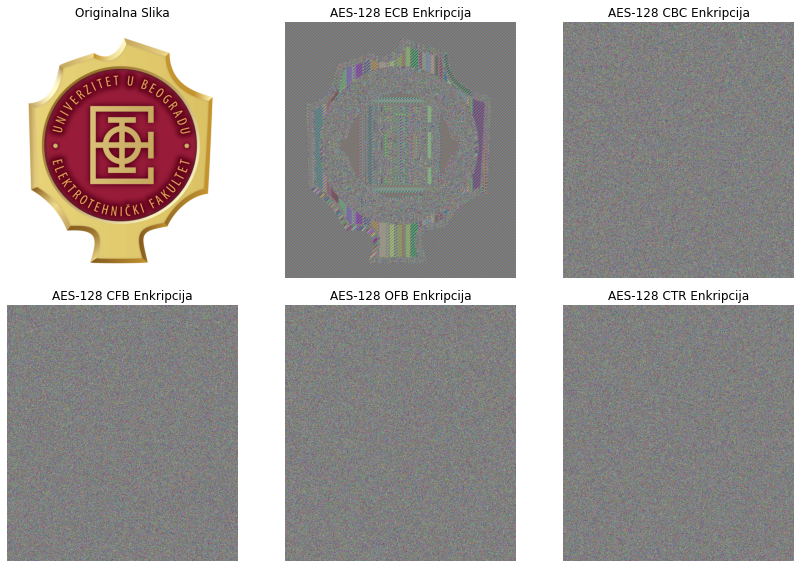
\includegraphics[width=0.9\columnwidth]{chapters/pictures/Modovi_rada_AES.png}
    \caption[AES-128 šifrovanje slike u različitim režimima rada]{AES-128 šifrovanje slike u različitim režimima rada. Preuzeto iz \cite{gavrilovic_diplomski}.}
    \label{fig:modovi_pecat}
\end{figure}

\subsubsection{CBC režim}

CBC (engl. \textit{Cipher Block Chaining}) otklanja slabost ECB režima ulančavanjem blokova, pri kome se svaki blok otvorenog teksta pre šifrovanja sabira sa prethodnim blokom šifrata,
\begin{equation}
    \mathrm{CT}_i = E_K(\mathrm{PT}_i \oplus \mathrm{CT}_{i-1}), \qquad \mathrm{CT}_0 = IV,
\end{equation}
gde je $IV$ nasumični inicijalizacioni vektor. Identični blokovi otvorenog teksta sada daju različite šifrate, ali se cena plaća upravo u onome što je za hardver najvažnije, u propusnosti. Šifrovanje bloka $i$ ne može početi pre nego što se završi blok $i-1$. Povratna sprega onemogućava protočnu obradu, pa AES jezgro sa latencijom od $L$ taktova postiže tek jedan blok na svakih $L$ taktova, ma koliko resursa bilo na raspolaganju. Pored toga, CBC zahteva dopunu poruke do umnoška bloka i koristi i smer dešifrovanja.

\subsubsection{CTR režim}
\label{subsubsec:ctr_rezim}

CTR (engl. \textit{Counter}) režim ide drugim putem. Umesto ulančavanja podataka šifruje se niz vrednosti brojača, a dobijeni pseudoslučajni niz sabira sa otvorenim tekstom,
\begin{equation}
    \mathrm{CT}_i = \mathrm{PT}_i \oplus E_K(IV \,\|\, i),
    \label{eq:ctr_generic}
\end{equation}
čime se blok šifra efektivno pretvara u protočnu šifru, a šema režima prikazana je na slici \ref{fig:ctr_sema}.

\begin{figure}[H]
\centering
\resizebox{0.8\textwidth}{!}{
\begin{tikzpicture}
    \node (cb1) [blokdata, minimum width=2.4cm] {$IV \,\|\, 1$};
    \node (ek1) [blokkripto, below=0.7cm of cb1, minimum width=2.4cm] {$E_K$};
    \node (xor1) [circle, draw=black, thick, below=0.7cm of ek1, inner sep=2pt] {$\oplus$};
    \node (p1) [blokdata, left=1cm of xor1, minimum width=1.4cm] {$\mathrm{PT}_1$};
    \node (c1) [blokrezultat, below=0.7cm of xor1, minimum width=1.4cm] {$\mathrm{CT}_1$};
    \draw [strelica] (cb1) -- (ek1);
    \draw [strelica] (ek1) -- (xor1);
    \draw [strelica] (p1) -- (xor1);
    \draw [strelica] (xor1) -- (c1);

    \node (cb2) [blokdata, right=2.4cm of cb1, minimum width=2.4cm] {$IV \,\|\, 2$};
    \node (ek2) [blokkripto, below=0.7cm of cb2, minimum width=2.4cm] {$E_K$};
    \node (xor2) [circle, draw=black, thick, below=0.7cm of ek2, inner sep=2pt] {$\oplus$};
    \node (p2) [blokdata, left=1cm of xor2, minimum width=1.4cm] {$\mathrm{PT}_2$};
    \node (c2) [blokrezultat, below=0.7cm of xor2, minimum width=1.4cm] {$\mathrm{CT}_2$};
    \draw [strelica] (cb2) -- (ek2);
    \draw [strelica] (ek2) -- (xor2);
    \draw [strelica] (p2) -- (xor2);
    \draw [strelica] (xor2) -- (c2);

    \node (dots) [right=1.2cm of ek2] {\Huge $\cdots$};
\end{tikzpicture}
}
\caption{CTR režim rada: blokovi se obrađuju nezavisno i paralelno}
\label{fig:ctr_sema}
\end{figure}

Svojstva CTR režima čine ga idealnim polazištem za hardver visoke propusnosti. Blokovi su potpuno nezavisni, jer brojački blok ne zavisi od podataka, pa je moguća i savršena protočnost i paralelizam. Poruka ne zahteva dopunu, jer se od poslednjeg bloka pseudoslučajnog niza uzima tačno onoliko bitova koliko je potrebno. Uz to, dešifrovanje je identičan postupak. Primalac istim ključem i istim brojačkim blokovima proizvede isti pseudoslučajni niz i sabere ga sa šifratom, pa se blok šifra i pri dešifrovanju poziva samo u smeru šifrovanja, a inverzna šifra iz odeljka \ref{subsec:aes_dekripcija} nije potrebna. Kritičan zahtev je da se vrednost brojača nikada ne ponovi sa istim ključem.

\subsubsection{Od CTR do GCM}

CTR režim, međutim, ne pruža nikakvu zaštitu integriteta. Štaviše, izrazito je savitljiv (engl. \textit{malleable}). Pošto je $\mathrm{CT}_i = \mathrm{PT}_i \oplus ks_i$, ako Oskar promeni proizvoljan bit šifrata, promenio je tačno taj bit dešifrovanog teksta, predvidljivo i neprimetno. Šifrovana poruka se stoga u praksi mora štititi i kodom za autentifikaciju, a GCM je upravo standardizovan odgovor na tu potrebu, sa CTR režimom za poverljivost i GHASH funkcijom za integritet, uz obradu pridruženih podataka. Tabela \ref{tab:ctr_vs_gcm} sumira poređenje.

\begin{table}[H]
\caption{Poređenje CTR i GCM režima rada}
\centering
\resizebox{0.95\textwidth}{!}{
\begin{tabular}{|c|c|c|}
\hline
\rowcolor{gray!30}
Svojstvo & CTR & GCM \\
\hline
poverljivost & da & da \\
\hline
integritet i autentifikacija poruke & ne & da \\
\hline
pridruženi podaci (AAD) & ne & da \\
\hline
paralelna obrada blokova & da & \makecell{da za šifrovanje, a autentifikacija je serijska, jedno \\ množenje po bloku (odeljak \ref{subsubsec:ghash_paralelizacija})} \\
\hline
koristi samo smer šifrovanja & da & da \\
\hline
dodatni hardver & --- & množač u GF($2^{128}$) (GHASH) \\
\hline
\end{tabular}
}
\label{tab:ctr_vs_gcm}
\end{table}

\subsection{GCM režim rada}
\label{subsec:gcm_rezim}

GCM (engl. \textit{Galois/Counter Mode}) \cite{sp80038d, mcgrew_viega} je AEAD režim rada koji objedinjuje dva gradivna elementa: CTR režim šifrovanja, zadužen za poverljivost, i GHASH funkciju autentifikacije, zaduženu za integritet. Ulaz u GCM šifrovanje čine:
\begin{itemize}[itemsep=2pt]
    \item tajni ključ $K$ (u ovom radu 256-bitni),
    \item nonce vrednost $IV$, jedinstvena za svaku poruku šifrovanu istim ključem,
    \item otvoreni tekst $\mathrm{PT}$ (engl. \textit{plaintext}) proizvoljne dužine,
    \item pridruženi podaci $\mathrm{AAD}$, koji se ne šifruju, ali ulaze u autentifikaciju. Tipično su to zaglavlja mrežnih paketa, koja moraju ostati čitljiva usput, a ne smeju biti izmenjena.
\end{itemize}
Izlaz su šifrat $\mathrm{CT}$ (engl. \textit{ciphertext}), iste dužine kao $\mathrm{PT}$, i autentifikaciona oznaka $\mathrm{ICV}$ (engl. \textit{Integrity Check Value}).
\smallbreak
Postupak počinje izvođenjem dve vrednosti. Prva je heš potključ (engl. \textit{hash subkey}):
\begin{equation}
    H = E_K(0^{128}),
\end{equation}
dobijen šifrovanjem nultog bloka, koji parametrizuje GHASH funkciju, a druga je početni brojački blok $J_0$. Za preporučenu dužinu nonce vrednosti od 96 bitova formira se jednostavnim nadovezivanjem,
\begin{equation}
    J_0 = IV \,\|\, 0^{31} \,\|\, 1,
    \label{eq:j0}
\end{equation}
dok se za ostale dužine $IV$ izvodi GHASH funkcijom nad dopunjenim $IV$. Upravo zbog jednostavnosti izraza (\ref{eq:j0}) hardverske realizacije po pravilu fiksiraju dužinu nonce vrednosti na 96 bitova.

\subsubsection{CTR šifrovanje}

Otvoreni tekst deli se na $n = \lceil \mathrm{len}(\mathrm{PT})/128 \rceil$ blokova $\mathrm{PT}_1, \ldots, \mathrm{PT}_n$, pri čemu poslednji blok može biti nepotpun. \textit{Brojački blokovi} (engl. \textit{counter block}) $CB_i$ generišu se funkcijom $\mathrm{inc_{32}}$, koja inkrementira najnižih 32 bita bloka po modulu $2^{32}$, ne dirajući gornjih 96 bitova:
\begin{equation}
    CB_1 = \mathrm{inc_{32}}(J_0), \qquad CB_i = \mathrm{inc_{32}}(CB_{i-1}), \quad i = 2, \ldots, n.
\end{equation}
Svaki brojački blok se šifruje, a rezultat sabira operacijom XOR sa odgovarajućim blokom otvorenog teksta:
\begin{equation}
    \mathrm{CT}_i = \mathrm{PT}_i \oplus E_K(CB_i), \qquad i = 1, \ldots, n-1,
\end{equation}
dok se za poslednji, potencijalno nepotpun blok dužine $u$ bitova koristi samo najznačajnijih $u$ bitova šifrovanog brojača:
\begin{equation}
    \mathrm{CT}_n = \mathrm{PT}_n \oplus \mathrm{MSB}_u\big(E_K(CB_n)\big).
\end{equation}
Brojački niz počinje od $J_0$, ali šifrovanje podataka počinje tek od $CB_1$, jer sam $J_0$ nikada ne šifruje podatke, nego je njegov šifrat $E_K(J_0)$ rezervisan za masku autentifikacione oznake u izrazu (\ref{eq:gcm_tag}). Time nijedan blok pseudoslučajnog niza nije upotrebljen dvaput, jer se maska oznake ne poklapa ni sa jednim blokom koji štiti podatke. Grana za poverljivost je, dakle, običan CTR režim nad blokovima $CB_1, \ldots, CB_n$, pa za nju važe sva svojstva iz odeljka \ref{subsec:rezimi_rada_detaljno}, pre svega protočna obrada bez povratne sprege.

\subsubsection{GHASH funkcija}
\label{subsubsec:ghash}

Autentifikacija u GCM režimu zasniva se na funkciji GHASH, definisanoj nad poljem $\mathrm{GF}(2^{128})$ sa redukcionim polinomom:
\begin{equation}
    f(x) = x^{128} + x^7 + x^2 + x + 1.
    \label{eq:gcm_polinom}
\end{equation}
Blokovi poruke tumače se kao koeficijenti polinoma nad tim poljem, a sažetak je vrednost tog polinoma u tački $H$. Za niz 128-bitnih blokova $X_1, X_2, \ldots, X_m$ to znači:
\begin{equation}
    \mathrm{GHASH}_H(X) = X_1 \cdot H^m \oplus X_2 \cdot H^{m-1} \oplus \cdots \oplus X_m \cdot H.
    \label{eq:ghash_polinom}
\end{equation}
Pošto je $H$ tajan, Oskar ne zna u kojoj se tački polinom računa, pa ne može da nađe drugu poruku sa istom vrednošću. Konstrukcije ovog tipa u literaturi se zovu univerzalne heš funkcije (engl. \textit{universal hash function}). Za razliku od SHA-3, one nisu sigurne same po sebi, nego tek uz tajni parametar i jednokratnu masku.
\smallbreak
Izraz (\ref{eq:ghash_polinom}) se ne izračunava neposredno, jer bi tražio sve stepene $H^2, \ldots, H^m$, nego Hornerovom šemom, u kojoj se svaki blok sabere sa akumulatorom, a zbir pomnoži sa $H$:
\begin{equation}
    Y_0 = 0^{128}, \qquad Y_i = (Y_{i-1} \oplus X_i) \cdot H, \qquad \mathrm{GHASH}_H(X) = Y_m.
    \label{eq:ghash_horner}
\end{equation}
Time je po bloku potrebno jedno jedino množenje u polju, i to sa uvek istim činiocem $H$. Sekvencijalni tok izračunavanja prikazan je na slici \ref{fig:ghash_lanac}.
\smallbreak
Ostaje još jedan detalj zapisa. Standard \cite{sp80038d} bitove 128-bitnog bloka pridružuje stepenima ogledalski u odnosu na uobičajeni binarni zapis. Krajnji levi bit bloka je koeficijent uz $x^0$, a krajnji desni uz $x^{127}$. Na matematička svojstva polja to nema uticaja, a u hardveru se svodi na preuređenje veza na ulazu i izlazu množača, bez ijednog logičkog elementa. Jedini uslov je da ono bude dosledno sprovedeno.

\begin{figure}[H]
\centering
\resizebox{0.95\textwidth}{!}{
\begin{tikzpicture}
    \node (y0) [blokdata, minimum width=1.8cm] {$Y_0 = 0$};
    \node (xor1) [circle, draw=black, thick, right=0.9cm of y0, inner sep=2pt] {$\oplus$};
    \node (x1) [blokdata, above=0.7cm of xor1, minimum width=1.2cm] {$X_1$};
    \node (h1) [blokghash, right=0.9cm of xor1, minimum width=1.3cm] {$\cdot\, H$};
    \node (xor2) [circle, draw=black, thick, right=0.9cm of h1, inner sep=2pt] {$\oplus$};
    \node (x2) [blokdata, above=0.7cm of xor2, minimum width=1.2cm] {$X_2$};
    \node (h2) [blokghash, right=0.9cm of xor2, minimum width=1.3cm] {$\cdot\, H$};
    \node (xor3) [circle, draw=black, thick, right=0.9cm of h2, inner sep=2pt] {$\oplus$};
    \node (x3) [blokdata, above=0.7cm of xor3, minimum width=1.2cm] {$X_3$};
    \node (h3) [blokghash, right=0.9cm of xor3, minimum width=1.3cm] {$\cdot\, H$};
    \node (ym) [blokrezultat, right=0.9cm of h3, minimum width=1.4cm] {$Y_3$};
    \draw [strelica] (y0) -- (xor1);
    \draw [strelica] (x1) -- (xor1);
    \draw [strelica] (xor1) -- (h1);
    \draw [strelica] (h1) -- node[below] {\small $Y_1$} (xor2);
    \draw [strelica] (x2) -- (xor2);
    \draw [strelica] (xor2) -- (h2);
    \draw [strelica] (h2) -- node[below] {\small $Y_2$} (xor3);
    \draw [strelica] (x3) -- (xor3);
    \draw [strelica] (xor3) -- (h3);
    \draw [strelica] (h3) -- (ym);
\end{tikzpicture}
}
\caption{GHASH funkcija kao Hornerova šema}
\label{fig:ghash_lanac}
\end{figure} Ulazni niz GHASH funkcije formira se nadovezivanjem pridruženih podataka $\mathrm{AAD}$ i šifrata $\mathrm{CT}$, svakog dopunjenog nulama do umnoška 128 bitova, i završnog bloka koji sadrži 64-bitne zapise njihovih dužina:
\begin{equation}
    S = \mathrm{GHASH}_H\big(\mathrm{AAD} \,\|\, 0^{v} \,\|\, \mathrm{CT} \,\|\, 0^{w} \,\|\, \mathrm{len}_{64}(\mathrm{AAD}) \,\|\, \mathrm{len}_{64}(\mathrm{CT})\big).
    \label{eq:ghash_ulaz}
\end{equation}
gde su $v$ i $w$ najmanji brojevi nula koji dužine $\mathrm{AAD}$ i $\mathrm{CT}$ dovode do umnoška 128 bitova. Uključivanje dužina u poslednji blok sprečava napade produžavanjem i preraspodelom granice između $\mathrm{AAD}$ i $\mathrm{CT}$. Konačno, oznaka se dobija šifrovanjem vrednosti $S$ blokom $J_0$:
\begin{equation}
    \mathrm{ICV} = \mathrm{MSB}_t\big(E_K(J_0) \oplus S\big),
    \label{eq:gcm_tag}
\end{equation}
gde je $t$ dužina oznake (pun format je $t = 128$). Ovaj korak je i razlog zašto sama GHASH funkcija ne mora biti kriptografski sigurna. Vrednost $S$ nikada ne napušta jezgro nezaštićena, nego se sabira sa maskom $E_K(J_0)$, koja je za svaku poruku druga. Bez poznavanja ključa Oskar ne može izračunati tu masku, pa ni konstruisati ispravnu oznaku za izmenjenu poruku. Celokupan postupak GCM šifrovanja, sa CTR granom i GHASH granom kao odvojenim funkcionalnim celinama, prikazan je na slici \ref{fig:gcm_sema} na primeru poruke od dva bloka. Blok $L$ na slici je završni blok sa dužinama, $L = \mathrm{len}_{64}(\mathrm{AAD}) \,\|\, \mathrm{len}_{64}(\mathrm{CT})$, iz izraza (\ref{eq:ghash_ulaz}).

\begin{figure}[H]
\centering
\resizebox{0.95\textwidth}{!}{
\begin{tikzpicture}
    % CTR grana
    \node (iv) [blokdata, minimum width=2cm] {$IV$};
    \node (j0) [blokdata, right=1.4cm of iv, minimum width=2cm] {$J_0$};
    \node (cb1) [blokdata, right=2cm of j0, minimum width=2cm] {$CB_1$};
    \node (cb2) [blokdata, right=2cm of cb1, minimum width=2cm] {$CB_2$};
    \draw [strelica] (iv) -- node[above] {\small $\|\, 0^{31} 1$} (j0);
    \draw [strelica] (j0) -- node[above] {\small $\mathrm{inc_{32}}$} (cb1);
    \draw [strelica] (cb1) -- node[above] {\small $\mathrm{inc_{32}}$} (cb2);

    \node (ek0) [blokkripto, below=0.9cm of j0, minimum width=2cm] {$E_K$};
    \node (ek1) [blokkripto, below=0.9cm of cb1, minimum width=2cm] {$E_K$};
    \node (ek2) [blokkripto, below=0.9cm of cb2, minimum width=2cm] {$E_K$};
    \draw [strelica] (j0) -- (ek0);
    \draw [strelica] (cb1) -- (ek1);
    \draw [strelica] (cb2) -- (ek2);

    \node (xor1) [circle, draw=black, thick, below=0.9cm of ek1, inner sep=2pt] {$\oplus$};
    \node (xor2) [circle, draw=black, thick, below=0.9cm of ek2, inner sep=2pt] {$\oplus$};
    \node (p1) [blokdata, right=0.6cm of xor1, minimum width=1.1cm] {$\mathrm{PT}_1$};
    \node (p2) [blokdata, right=0.6cm of xor2, minimum width=1.1cm] {$\mathrm{PT}_2$};
    \draw [strelica] (ek1) -- (xor1);
    \draw [strelica] (ek2) -- (xor2);
    \draw [strelica] (p1) -- (xor1);
    \draw [strelica] (p2) -- (xor2);

    \node (c1) [blokrezultat, below=0.8cm of xor1, minimum width=1.4cm] {$\mathrm{CT}_1$};
    \node (c2) [blokrezultat, below=0.8cm of xor2, minimum width=1.4cm] {$\mathrm{CT}_2$};
    \draw [strelica] (xor1) -- (c1);
    \draw [strelica] (xor2) -- (c2);

    % GHASH grana
    \node (ghash) [blokghash, below=1.3cm of c1, xshift=2cm, minimum width=6.4cm, minimum height=1.1cm] {$\mathrm{GHASH}_H$};
    \node (aad) [blokdata, left=1.6cm of ghash, minimum width=1.1cm] {$\mathrm{AAD}$};
    \node (len) [blokdata, right=1.6cm of ghash, minimum width=1.1cm] {$L$};
    \draw [strelica] (c1) -- (ghash);
    \draw [strelica] (c2) -- (ghash);
    \draw [strelica] (aad) -- (ghash);
    \draw [strelica] (len) -- (ghash);

    \node (xort) [circle, draw=black, thick, below=0.9cm of ghash, inner sep=2pt] {$\oplus$};
    \draw [strelica] (ghash) -- node[right] {\small $S$} (xort);
    \draw [strelica] (ek0) |- node[below left, xshift=1.2cm] {\small $E_K(J_0)$} (xort);

    \node (tag) [blokrezultat, below=0.8cm of xort, minimum width=2.6cm] {$T = \mathrm{MSB}_t$};
    \draw [strelica] (xort) -- (tag);
\end{tikzpicture}
}
\caption{Blok šema GCM šifrovanja poruke od dva bloka: CTR grana (žuto/zeleno) i GHASH grana (cijan)}
\label{fig:gcm_sema}
\end{figure}

\begin{example}
Za poruku sa jednim blokom pridruženih podataka $\mathrm{AAD}_1$ i dva bloka šifrata $\mathrm{CT}_1, \mathrm{CT}_2$ ulazni niz ima četiri bloka, pa izraz (\ref{eq:ghash_polinom}) daje:
\begin{equation*}
    S = \mathrm{AAD}_1 \cdot H^4 \,\oplus\, \mathrm{CT}_1 \cdot H^3 \,\oplus\, \mathrm{CT}_2 \cdot H^2 \,\oplus\, L \cdot H,
\end{equation*}
gde je $L = \mathrm{len}_{64}(\mathrm{AAD}) \| \mathrm{len}_{64}(\mathrm{CT})$ završni blok sa dužinama. Isti rezultat Hornerova šema (\ref{eq:ghash_horner}) dobija u četiri koraka, sa jednim množenjem po koraku.
\end{example}

\subsubsection{Množenje u \texorpdfstring{$\mathrm{GF}(2^{128})$}{GF(2\^{}128)}}
\label{subsubsec:gf128_mnozenje}

Sve što GCM režim traži od aritmetike svodi se na jednu operaciju, množenje dva elementa polja $\mathrm{GF}(2^{128})$ iz izraza (\ref{eq:ghash_horner}). Sabiranje je XOR i praktično je besplatno, a šifrovanje obavlja AES, pa je ovo množenje jedina netrivijalna računska operacija u režimu. Kako se izvršava po jednom za svaki blok poruke, ono i određuje gornju granicu propusnosti autentifikacije.
\smallbreak
Množenje se razlaže na dva koraka: množenje polinoma bez prenosa, koje daje nesvedeni proizvod stepena do 254, i redukciju po modulu polinoma (\ref{eq:gcm_polinom}).
\smallbreak
\textit{Množenje polinoma.} Školski postupak, u kome se svaki bit jednog činioca množi svakim bitom drugog, traži $128^2 = 16\,384$ parcijalnih proizvoda. U polju karakteristike 2 svaki od njih je jedno logičko I kolo, a njihovo sabiranje jedno stablo XOR kola. Kvadratni rast sa dužinom operanda čini ovaj pristup izuzetno rasipnim za polja ovakve veličine.
\smallbreak
Povoljniji postupak daje Karatsubin algoritam \cite{karatsuba1962}. Operandi se rastave na polovine, $A = A_1 x^{n/2} + A_0$ i $B = B_1 x^{n/2} + B_0$, pa je proizvod:
\begin{equation}
    A \cdot B = A_1B_1\, x^{n} \;\oplus\; \big[(A_1 \oplus A_0)(B_1 \oplus B_0) \oplus A_1B_1 \oplus A_0B_0\big]\, x^{n/2} \;\oplus\; A_0B_0.
    \label{eq:karatsuba_teorija}
\end{equation}
Raspored tri proizvoda po rezultatu prikazan je na slici \ref{fig:karatsuba_ideja}. Svaki je širok najviše $n-1$ bitova, a pomereni su za $0$, $n/2$ i $n$ mesta, pa se susedni preklapaju po polovini svoje dužine. Ključna je ušteda u srednjem članu. Po školskom postupku on iznosi $A_1B_0 \oplus A_0B_1$ i traži dva množenja. U izrazu (\ref{eq:karatsuba_teorija}) dobija se iz jednog novog proizvoda i dva koja su za spoljne članove ionako već izračunata. Umesto četiri množenja polovina potrebna su, dakle, tri, po cenu nekoliko dodatnih sabiranja.
\smallbreak
Primenjen rekurzivno, postupak svodi složenost sa $\mathcal{O}(n^2)$ na $\mathcal{O}\big(n^{\log_2 3}\big) \approx \mathcal{O}(n^{1{,}585})$.

\begin{figure}[H]
\centering
\resizebox{0.92\textwidth}{!}{
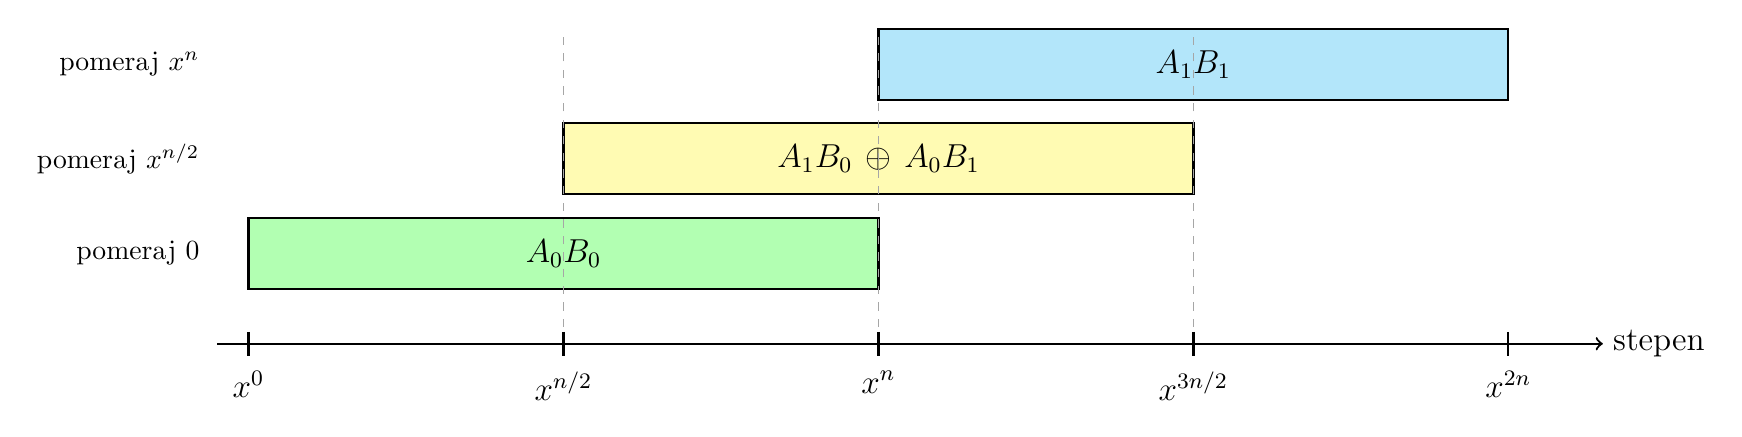
\begin{tikzpicture}[font=\large]
    % tri proizvoda polovina, svaki sirok n, pomeren za 0, n/2 i n
    \draw [draw=black, thick, fill=cyan!30]   (8,3.1) rectangle (16,4.0)
        node[midway] {$A_1 B_1$};
    \draw [draw=black, thick, fill=yellow!30] (4,1.9) rectangle (12,2.8)
        node[midway] {$A_1 B_0 \,\oplus\, A_0 B_1$};
    \draw [draw=black, thick, fill=green!30]  (0,0.7) rectangle (8,1.6)
        node[midway] {$A_0 B_0$};
    % isprekidane linije koje vezuju pomeraje za osu
    \foreach \x in {4,8,12}{
        \draw [dashed, gray!70] (\x,0) -- (\x,4.0);
    }
    % osa stepena
    \draw [->, thick] (-0.4,0) -- (17.2,0) node[right] {stepen};
    \foreach \x/\l in {0/$x^{0}$, 4/$x^{n/2}$, 8/$x^{n}$, 12/$x^{3n/2}$, 16/$x^{2n}$}{
        \draw [thick] (\x,0.15) -- (\x,-0.15) node[below=2pt] {\l};
    }
    % oznake pomeraja
    \node [anchor=east, font=\normalsize] at (-0.5,1.15) {pomeraj $0$};
    \node [anchor=east, font=\normalsize] at (-0.5,2.35) {pomeraj $x^{n/2}$};
    \node [anchor=east, font=\normalsize] at (-0.5,3.55) {pomeraj $x^{n}$};
\end{tikzpicture}
}
\caption{Karatsubin algoritam}
\label{fig:karatsuba_ideja}
\end{figure}

Za binarna polja ovaj algoritam je povoljniji nego za obične cele brojeve, i to iz dva razloga. Prvi je da dodatna sabiranja koja Karatsubin postupak unosi ovde nisu sabiranja sa prenosom, nego XOR operacije, jedan logički nivo, bez prostiranja prenosa duž reči. Drugi je da se time cela struktura svodi na čistu kombinacionu mrežu, čija dubina raste logaritamski sa $n$. Dubina rekurzije je pritom kompromis između broja osnovnih množenja i dubine mreže. Sistematska analiza data je u \cite{weimerskirch_paar}.
\smallbreak
\textit{Redukcija.} Nesvedeni proizvod stepena do 254 vraća se u polje smenom $x^{128} = x^7 + x^2 + x + 1$, koja sledi neposredno iz (\ref{eq:gcm_polinom}). Svaki postavljen bit iznad stepena 127 tako se preslikava u najviše četiri niža stepena. Pošto su svi članovi redukcionog polinoma osim vodećeg ispod $x^8$, jedan prolaz spušta najviši stepen sa 254 na 133, a drugi na 12. Dva prolaza su, dakle, dovoljna, i oba su plitke mreže XOR kola. Malobrojni i niski članovi redukcionog polinoma upravo su ono što redukciju čini ovako plitkom, i po tome se ovakvi polinomi i biraju za kriptografska polja.
\smallbreak
Konkretna dubina rekurzije, broj osnovnih množenja i uticaj na kritičnu putanju u realizaciji ovog rada dati su u odeljku \ref{subsec:hw_ghash}.

\subsubsection{Dešifrovanje i provera oznake}

Pri dešifrovanju primalac najpre istim postupkom, nad primljenim šifratom i pridruženim podacima, izračunava očekivanu oznaku $\mathrm{ICV}'$, pa je poredi sa primljenom oznakom $\mathrm{ICV}$. Poruka se prihvata samo ako je $\mathrm{ICV}' = \mathrm{ICV}$, a dešifrovani sadržaj ne sme biti prosleđen dalje, ni primaocu ni bilo kom potrošaču nizvodno, pre nego što provera uspe. Realizacije koje poruku obrađuju u prolazu, ne zadržavajući ceo njen sadržaj, taj zahtev ispunjavaju tako što uz dešifrovani tok isporuče i ishod provere na kraju poruke, pa obaveza odbacivanja prelazi na prvog potrošača -- tako postupa i realizacija iz poglavlja \ref{ch:hardver}. Sam šifrat se dešifruje identičnim CTR postupkom kao pri šifrovanju, jer operacija XOR sa istim pseudoslučajnim nizom poništava svoje dejstvo. Otuda i posledica najavljena u odeljku \ref{subsec:aes_dekripcija}: i pri dešifrovanju se šifra poziva samo u smeru šifrovanja, a razlika postoji jedino u završnom koraku, koji oznaku u jednom slučaju generiše, a u drugom proverava.

\subsubsection{Paralelizacija GHASH funkcije}
\label{subsubsec:ghash_paralelizacija}

Za razliku od CTR grane, koja je savršeno paralelna, Hornerova šema (\ref{eq:ghash_horner}) nameće striktno sekvencijalnu obradu. Svaki blok zahteva jedno množenje sa $H$ pre prihvatanja narednog, pa jedan množač koji množenje izvršava u $c$ taktova ograničava propusnost na jedan blok svakih $c$ taktova. Ovo ograničenje, međutim, pripada načinu izračunavanja, a ne samoj funkciji. Polinomijalni oblik (\ref{eq:ghash_polinom}) nema nikakvu povratnu spregu, pa se grupisanjem po $p$ uzastopnih blokova, uz unapred izračunate stepene $H^2, H^3, \ldots, H^p$, dobija:
\begin{equation}
    Y_{i} = \big(Y_{i-p} \oplus X_{i-p+1}\big) \cdot H^{p} \,\oplus\, X_{i-p+2} \cdot H^{p-1} \,\oplus\, \cdots \,\oplus\, X_{i} \cdot H,
\end{equation}
pa $p$ paralelnih množača obrađuje $p$ blokova istovremeno, umnožavajući propusnost autentifikacije $p$ puta. Slika \ref{fig:ghash_paralelno} prikazuje strukturu za $p=2$. Dva množača rade paralelno, jedan sa stepenom $H^2$ nad akumulatorom i neparnim blokom, drugi sa $H$ nad parnim blokom, a njihovi rezultati se sabiraju u novi akumulator.

\begin{figure}[H]
\centering
\resizebox{0.75\textwidth}{!}{
\begin{tikzpicture}
    \node (ym2) [blokdata, minimum width=1.8cm] {$Y_{i-2}$};
    \node (xora) [circle, draw=black, thick, right=1cm of ym2, inner sep=2pt] {$\oplus$};
    \node (xm1) [blokdata, above=0.7cm of xora, minimum width=1.4cm] {$X_{i-1}$};
    \node (h2) [blokghash, right=1cm of xora, minimum width=1.6cm] {$\cdot\, H^2$};
    \node (h1) [blokghash, below=1.4cm of h2, minimum width=1.6cm] {$\cdot\, H$};
    \node (xi) [blokdata, left=1cm of h1, minimum width=1.4cm] {$X_i$};
    \node (xorb) [circle, draw=black, thick, right=1.4cm of h2, yshift=-1.05cm, inner sep=2pt] {$\oplus$};
    \node (yi) [blokrezultat, right=1cm of xorb, minimum width=1.4cm] {$Y_i$};
    \draw [strelica] (ym2) -- (xora);
    \draw [strelica] (xm1) -- (xora);
    \draw [strelica] (xora) -- (h2);
    \draw [strelica] (xi) -- (h1);
    \draw [strelica] (h2) -- (xorb);
    \draw [strelica] (h1) -- (xorb);
    \draw [strelica] (xorb) -- (yi);
\end{tikzpicture}
}
\caption{Paralelizovani GHASH za $p=2$}
\label{fig:ghash_paralelno}
\end{figure}

Broj množača i latencija množenja izbor su realizacije. Kompromis za sistem iz ovog rada kvantifikovan je u odeljku \ref{subsec:hw_ghash_cycles}.

\subsection{Sigurnosna svojstva i ograničenja}
\label{subsec:gcm_sigurnost}

GCM režim nasleđuje snagu AES algoritma, ali njegova sigurnost kritično zavisi od pravilne upotrebe nonce vrednosti, jer se ista vrednost $IV$ nikada ne sme upotrebiti dva puta sa istim ključem. Ponavljanje nonce vrednosti u CTR režimu dovodi do ponavljanja pseudoslučajnog niza, čime Oskar dobija XOR dva otvorena teksta. Kod GCM-a posledice su još teže, jer razlika dve oznake dobijene istim brojačkim blokom daje jednačinu po potključu $H$, iz koje se dobija svega nekoliko kandidata, a u praktičnim slučajevima i sam $H$. Time postaje moguće falsifikovanje oznaka za proizvoljne poruke \cite{joux_gcm}. Zbog toga je generisanje nonce vrednosti, tipično brojačem ili kombinacijom fiksnog polja i brojača poruka, sastavni deo pravilne upotrebe režima i mora biti pažljivo rešeno i na nivou hardverskog interfejsa akceleratora.
\smallbreak
Pored jedinstvenosti nonce vrednosti, standard \cite{sp80038d} ograničava dužinu poruke na najviše $2^{39}-256$ bitova, propisuje minimalne preporučene dužine oznake u zavisnosti od primene i ograničava ukupan broj poziva sa istim ključem. U sistemu realizovanom u ovom radu jedan ključ sesije štiti sav saobraćaj svoje sesije. Jedinstvenost nonce vrednosti obezbeđuje deterministička konstrukcija sa brojačem poruka, koja ujedno prostorom brojača ograničava broj poziva sa istim ključem, a sveža ECDH razmena sa izvođenjem novih ključeva dostupna je u svakom trenutku kada sesiju treba obnoviti. Navedena ograničenja time se poštuju konstrukcijom protokola.
